\documentclass[conference]{IEEEtran}

\usepackage{cite}
\usepackage{amsmath,amssymb,amsfonts}
\usepackage{graphicx}
\usepackage{textcomp}
\usepackage{xcolor}
\usepackage{booktabs}
\usepackage{url}
\usepackage{float}
\usepackage{placeins}

\graphicspath{{figures/}}

% Allow more floats per page and reduce minimum text fraction
\renewcommand{\topfraction}{0.9}
\renewcommand{\bottomfraction}{0.8}
\renewcommand{\textfraction}{0.07}
\renewcommand{\floatpagefraction}{0.85}
\setcounter{topnumber}{4}
\setcounter{bottomnumber}{2}
\setcounter{totalnumber}{6}

\begin{document}

\title{Biomedical Text Embeddings Weakly Capture Chromatin Accessibility
Similarity: A Large-Scale Measurement Study}

\author{
  \IEEEauthorblockN{Joshua Song}
  \IEEEauthorblockA{
    Department of Biomedical Engineering \\
    University of Illinois Chicago \\
    joshuajsong@gmail.com
  }
}

\maketitle

\begin{abstract}
The extent to which biomedical text metadata can serve as a proxy for
chromatin accessibility similarity remains unknown. We conducted a systematic
measurement study comparing pairwise similarity structures derived from 11
distinct embedding types---including Atacformer, regulatory potential (RP),
four biomedical language models, TF-IDF, and a random baseline---across
32,245 human ATAC-seq experiments from ChIP-Atlas. Using Spearman rank
correlation, Mantel permutation tests, and top-$k$ neighborhood overlap, we
find that text embeddings of experimental metadata show weak but statistically
significant correlation with Atacformer-derived chromatin similarity
($\rho = 0.06$ at cell-type level; $\rho = 0.25$--$0.28$ at full scale).
Strikingly, TF-IDF matches or outperforms all neural language models,
indicating that surface-level vocabulary---not semantic understanding---drives
this correlation. Biomedical language models marginally outperform a
general-purpose encoder, but neither approach overcomes the TF-IDF baseline.
Furthermore, text embeddings share only 2--3\% of nearest neighbors with
Atacformer but 20--23\% with regulatory potential, revealing that text captures
cell-type-level clustering recoverable from metadata but not the richer
chromatin landscape encoded by Atacformer. These results establish quantitative
bounds on the utility of text metadata as a proxy for chromatin similarity and
motivate continued development of chromatin-specific representation models.
\end{abstract}

\begin{IEEEkeywords}
ATAC-seq, chromatin accessibility, text embeddings, biomedical NLP,
representation learning, measurement study
\end{IEEEkeywords}


% ── Introduction ──────────────────────────────────────────────────────────────
\section{Introduction}

The rapid growth of epigenomics databases such as ChIP-Atlas~\cite{chipatlas},
ENCODE~\cite{encode}, and Roadmap Epigenomics~\cite{roadmap} has produced tens
of thousands of ATAC-seq experiments across diverse human cell types and
conditions. Organizing, retrieving, and comparing these experiments requires
similarity measures that reflect the underlying biology. A natural question
arises: to what extent can text metadata associated with experiments---cell
type labels, experimental descriptions, and publication titles---serve as a
proxy for chromatin accessibility similarity?

This question has direct practical implications. If text embeddings closely
approximate chromatin-based similarity, they could enable natural-language
retrieval and annotation of ATAC-seq data without access to the raw signal,
potentially democratizing the use of large epigenomics repositories.
Conversely, if agreement is limited, such analyses motivate continued
investment in chromatin-specific representation learning and highlight the
irreducible information content of the chromatin signal itself.

Recent advances in biomedical natural language processing have produced
powerful text encoders pretrained on large biomedical corpora.
PubMedBERT~\cite{pubmedbert} is pretrained from scratch on PubMed abstracts
and full-text articles. SapBERT~\cite{sapbert} and MedCPT~\cite{medcpt} are
both initialized from a pretrained PubMedBERT checkpoint and further
fine-tuned for different objectives: SapBERT via self-alignment on UMLS
synonym pairs, and MedCPT via contrastive learning on PubMed search logs.
These models achieve strong performance on biomedical entity recognition,
relation extraction, and information retrieval, yet whether their semantic
representations capture the biological relationships encoded in chromatin
accessibility data has not been systematically evaluated.

Atacformer~\cite{atacformer} is a transformer trained on ATAC-seq data using
triplet margin loss to produce experiment-level embeddings that cluster by cell
type and chromatin state. Regulatory potential (RP)~\cite{lisa2} provides a
complementary, functional-genomics-derived signal: a gene-activation-weighted
summary of chromatin accessibility indexed by gene transcription start sites.

We present a large-scale measurement study comparing pairwise similarity
structures from 11 embedding types across 32,245 curated human ATAC-seq
experiments. We treat this as a measurement problem where both agreement and
disagreement constitute informative scientific findings.

% ── Methods ───────────────────────────────────────────────────────────────────
\section{Methods}

Fig.~\ref{fig:schematic} summarizes the overall study design: chromatin-based
embeddings (Atacformer, RP) and text-based embeddings (biomedical and general
language models, TF-IDF, random) are computed for each experiment, converted
into pairwise similarity matrices at two levels of aggregation, and compared
using the three metrics described in Section~\ref{sec:metrics}.

\begin{figure*}[!t]
  \centering
  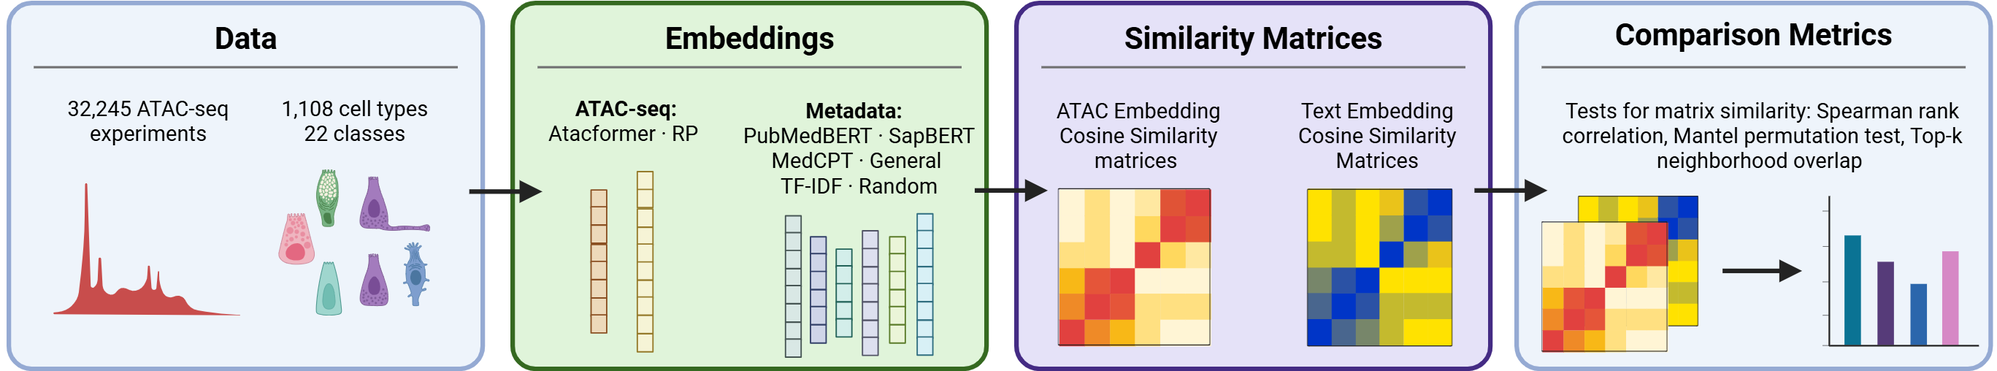
\includegraphics[width=\linewidth]{fig1.png}
  \caption{Study design. ATAC-seq experiments are embedded
  using chromatin-based models (Atacformer, RP), text encoders (biomedical and
  general language models, TF-IDF), and a random baseline. Pairwise cosine
  similarity matrices are computed at cell-type-aggregated and full-dataset
  levels and compared using three complementary metrics.}
  \label{fig:schematic}
\end{figure*}

\subsection{Dataset}

We obtained 48,822 human ATAC-seq experiments from ChIP-Atlas
(hg38 assembly)~\cite{chipatlas}. We removed 16,567 experiments with
corrupted or empty BED files and 10 experiments producing zero regulatory
potential signal near gene TSSs, yielding a curated set of 32,245
experiments spanning 1,108 cell types and 22 cell type
classes. Cell type labels were normalized using fuzzy string matching
(RapidFuzz, token\_sort\_ratio $\geq 82$), Jaccard token overlap
($\geq 0.60$), and acronym detection, generating 342 candidate merge pairs
of which 11 were applied after manual review (Table~\ref{tab:remap}).

\begin{table}[!t]
  \centering
  \caption{Cell-type label remaps applied after manual review (11 of 342
  candidate merge pairs identified by fuzzy string matching, Jaccard token
  overlap, and acronym detection).}
  \label{tab:remap}
  \resizebox{\columnwidth}{!}{%
  \begin{tabular}{lll}
    \toprule
    Original label & Canonical label & Method \\
    \midrule
    Leukemic stem cells                 & Leukemic stem cell              & Fuzzy-match review \\
    Retinal organoids                   & Retinal organoid                & Fuzzy-match review \\
    Glioblstoma stem cell                & Glioblastoma stem cells          & Fuzzy-match review \\
    Neuronal progenitor cels            & Neural progenitor cells          & Fuzzy-match review \\
    Ovarion cancer                      & Ovarian cancer                   & Fuzzy-match review \\
    Plasma Cells                        & Plasma B-cells                   & Fuzzy-match review \\
    Adipose-derived stem cells          & Adipose stem cells                & Fuzzy-match review \\
    Plasma                              & Plasma Cells                     & Fuzzy-match review \\
    Diffuse intrinsic pontine glioma    & DIPG                              & Fuzzy-match review \\
    Peripheral blood mononuclear cells  & PBMC                              & Fuzzy-match review \\
    Acute T cell leukemia               & T-ALL                             & Manual correction \\
    \bottomrule
  \end{tabular}}
\end{table}

\subsection{Atacformer Embeddings}

We encoded each experiment using \url{databio/atacformer-base-hg38}
(AtacformerForCellClustering)~\cite{atacformer}, a transformer trained with
triplet margin loss. Peak BED files were tokenized using the gtars Tokenizer
with a vocabulary of 890K genomic regions. Up to 1,024 randomly sampled peak
tokens were mean-pooled to produce a 192-dimensional embedding per experiment.

\subsection{Regulatory Potential Embeddings}

We computed RP for each experiment using a LISA2-style exponential decay
model~\cite{lisa2}, weighting chromatin peaks by distance to gene TSSs
(half-width 10 kb) with exon-aware upweighting. Each experiment was mapped
to a 40,772-dimensional vector indexed by hg38 autosomal gene TSSs.

\subsection{Text Embeddings}

For each experiment we constructed a full metadata string by concatenating
available fields: \{cell\_type\}. \{cell\_type\_class\}.
\{cell\_type\_description\}. \{title\}. We embedded this string using four
encoders, all of which produce 768-dimensional embeddings:
PubMedBERT~\cite{pubmedbert}
(\url{microsoft/BiomedNLP-BiomedBERT-base-uncased-abstract-fulltext}, mean
pooling), SapBERT~\cite{sapbert}
(\url{cambridgeltl/SapBERT-from-PubMedBERT-fulltext}, CLS pooling),
MedCPT~\cite{medcpt} (\url{ncbi/MedCPT-Query-Encoder}, mean
pooling), and a General encoder~\cite{mpnet}
(\url{sentence-transformers/all-mpnet-base-v2}, mean pooling). To isolate
the contribution of cell type identity, we also encoded each experiment using
only the cell type name string with all four models (cell-type-name-only
ablation). We additionally computed TF-IDF embeddings (top 2,048
features, sublinear TF, 2,048-dimensional) and a random Gaussian
baseline (192-d, fixed seed).

\subsection{Similarity Matrices and Comparison Metrics}
\label{sec:metrics}

For each embedding type we computed pairwise cosine similarity matrices at two
levels: (1)~cell-type aggregated---mean-pooling embeddings within
each cell type ($1{,}108 \times 1{,}108$); and (2)~full
dataset---all 32,245 experiments ($32{,}245 \times 32{,}245$). All
embeddings were corpus-centered prior to similarity computation to correct for
anisotropy in transformer mean-pool representations.

We quantified agreement using four metrics:
\begin{enumerate}
  \item Spearman rank correlation ($\rho$) on upper-triangle edge weights.
  \item Mantel permutation test (1,000 permutations) for empirical
        $p$-values at the cell-type level.
  \item Bootstrap confidence intervals for $\rho$ (1,000 resamples
        of cell types/experiments, with 50,000 randomly sampled pairs per
        resample), reported at both the cell-type and full-dataset scale as a
        scale-independent measure of effect-size precision.
  \item Top-$k$ neighborhood overlap: mean fraction of shared top-$k$
        nearest neighbors, $k \in \{5, 10, 20, 50\}$.
\end{enumerate}

All analyses were conducted with both Atacformer and RP as reference
structures. Mantel tests were GPU-accelerated on an NVIDIA GB10 GPU
($\sim$30~s per condition vs.\ $\sim$38~min on CPU).

\subsection{Decomposing LLM Signal from TF-IDF}

To determine whether neural language models encode biological information
beyond surface-level vocabulary overlap, we conducted three complementary
analyses comparing the full-text LLM embeddings against TF-IDF at both the
cell-type-aggregated and full 32,245-experiment levels.

Pairwise similarity scatter. For each LLM, we sampled up to 30,000
random experiment pairs and plotted TF-IDF pairwise similarity against LLM
pairwise similarity, coloring each point by Atacformer similarity. Points
above the diagonal indicate pairs where the LLM assigns higher similarity than
TF-IDF; points below indicate the reverse. The Spearman correlation between
TF-IDF and LLM similarity vectors was computed over the same sample.

Partial Spearman correlation. We computed the partial Spearman
rank correlation of each LLM similarity matrix with Atacformer, controlling
for TF-IDF:
\begin{equation}
  \rho_{LM,AC \mid TF} =
    \frac{\rho_{LM,AC} - \rho_{LM,TF}\,\rho_{AC,TF}}
         {\sqrt{(1-\rho_{LM,TF}^{2})(1-\rho_{AC,TF}^{2})}}
\end{equation}
where $\rho_{X,Y}$ denotes the Spearman correlation of the upper-triangle
edge weights of matrices $X$ and $Y$. At the full scale, correlations were
estimated on a random subsample of $2 \times 10^6$ pairs from the
${\sim}520$M-element upper triangle. A positive partial correlation indicates
that the LLM encodes biological structure beyond vocabulary overlap; a value
near zero or negative indicates its Atacformer alignment is fully explained
by TF-IDF.

Cross top-$k$ neighborhood overlap. For each LLM and each
$k \in \{5, 10, 20, 50\}$, we computed the mean fraction of top-$k$ LLM
nearest neighbors that are also top-$k$ TF-IDF nearest neighbors, using the
same topk\_overlap procedure described above. High overlap indicates
the LLM's local structure recapitulates TF-IDF; low overlap indicates
genuinely distinct neighbor assignments.

% ── Results ───────────────────────────────────────────────────────────────────
\section{Results}

\subsection{Text Embeddings Show Weak but Significant Alignment with Atacformer}

Sanity checks confirmed that Atacformer and RP produce biologically coherent
similarity structures, with immune, neural, and cancer cell types forming
distinct clusters, while text-based embeddings show coarser organization
(Fig.~\ref{fig:s1}).

\begin{figure*}[!t]
  \centering
  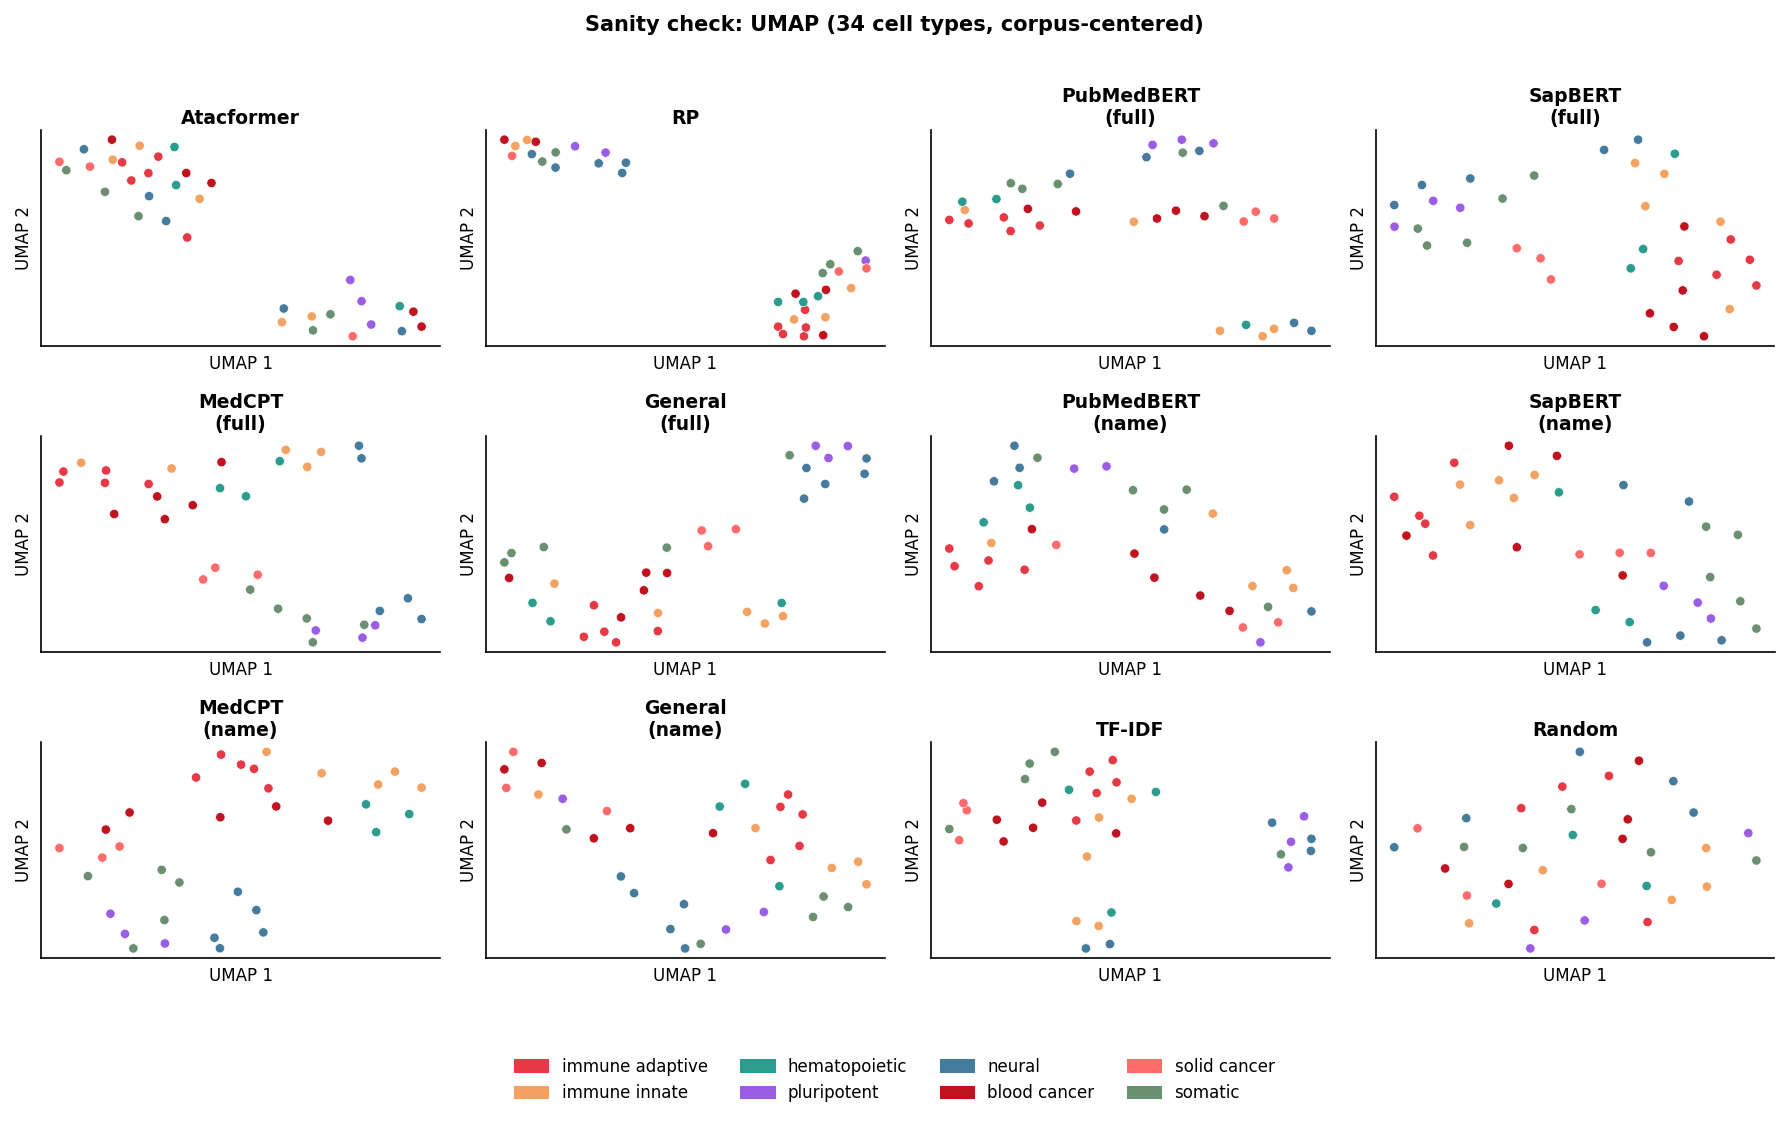
\includegraphics[width=\linewidth]{figS1a.png}
  \vspace{6pt}
  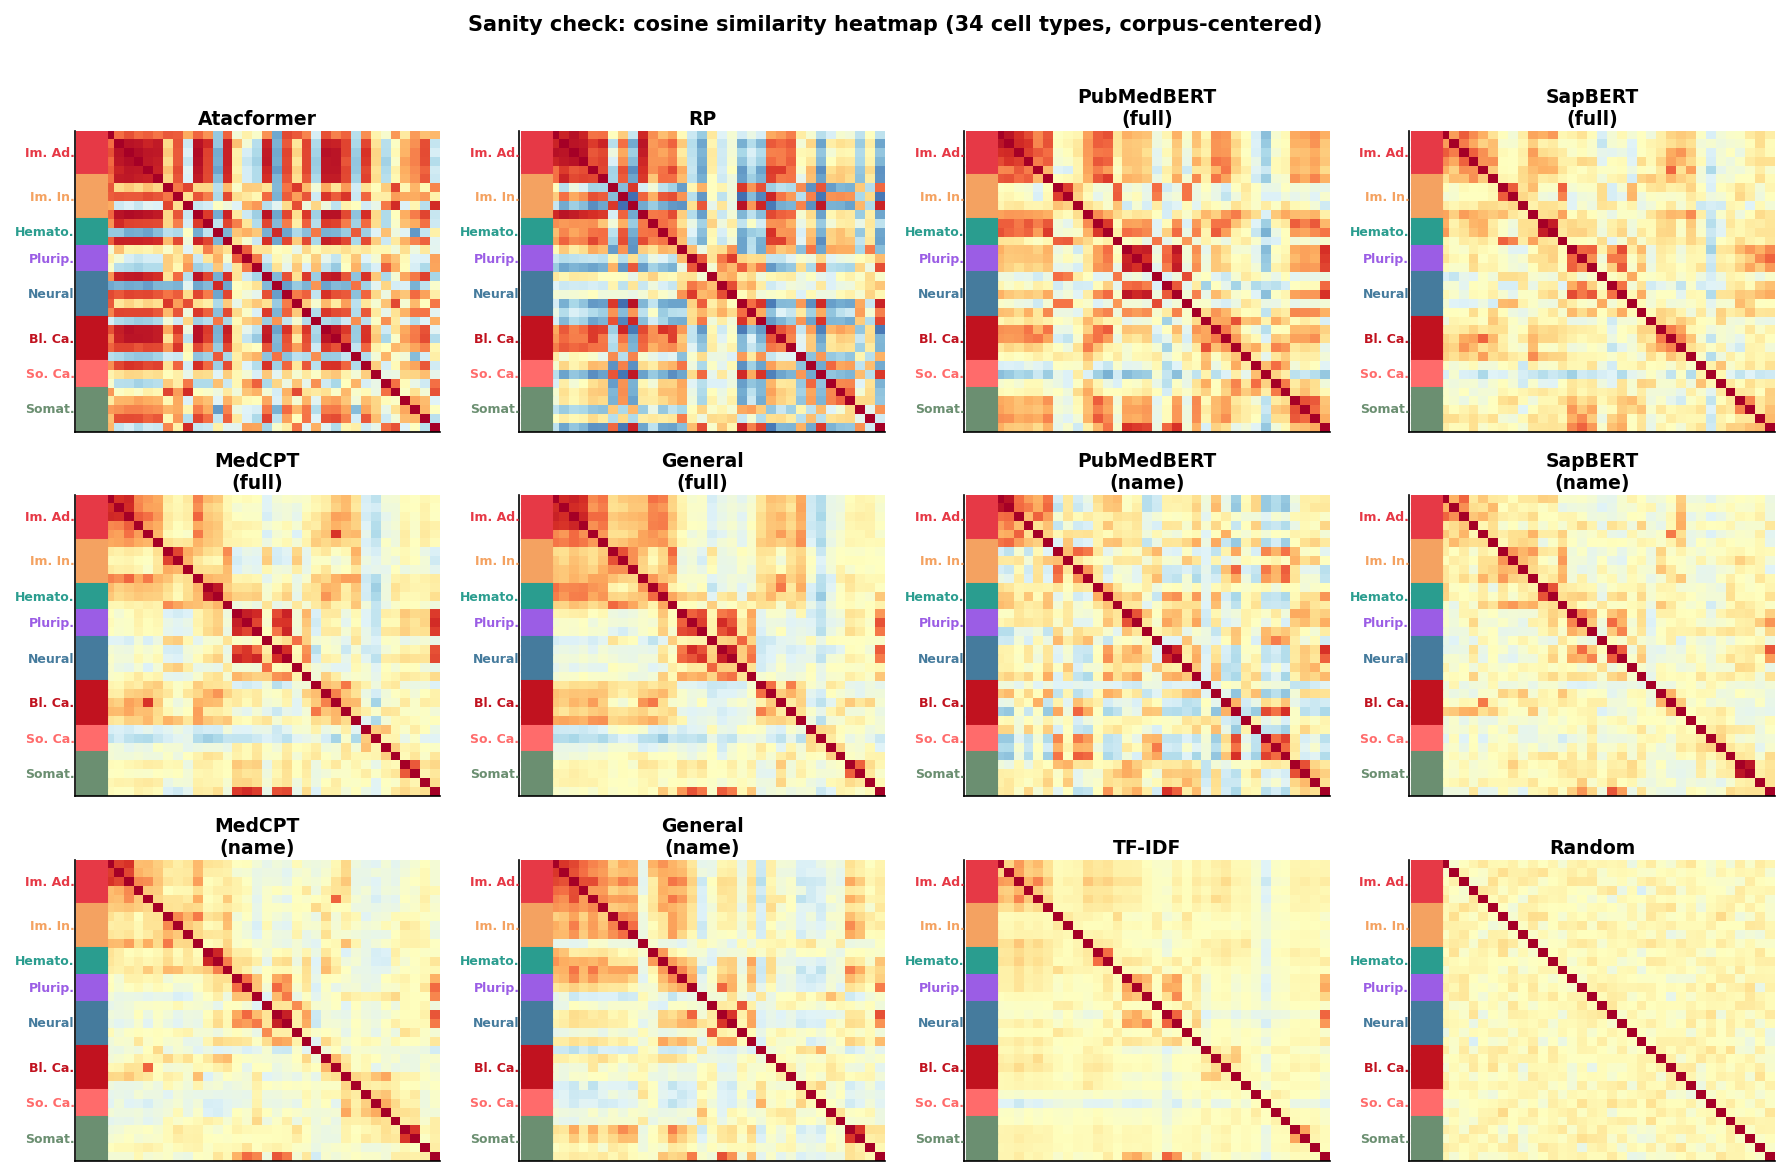
\includegraphics[width=\linewidth]{figS1b.png}
  \caption{Sanity check UMAP projections (top) and cosine
  similarity heatmaps (bottom) for all 12 embedding conditions over 34
  representative cell types. Atacformer and RP show biologically coherent
  lineage clustering; text-based models show coarser, cell-type-level
  organization.}
  \label{fig:s1}
\end{figure*}

At the cell-type-aggregated level, all four full-text biomedical embeddings
showed weak but statistically significant Spearman rank correlation with
Atacformer (PubMedBERT: $\rho = 0.060$; SapBERT: $\rho = 0.057$;
MedCPT: $\rho = 0.035$; General: $\rho = 0.032$; all Mantel $p < 0.01$,
$N = 1{,}000$ permutations; Table~\ref{tab:spearman}). TF-IDF showed
comparable agreement ($\rho = 0.060$, $p < 0.001$). Critically,
cell-type-name-only variants of the same models showed no significant
correlation with Atacformer ($\rho \approx 0$, $p > 0.20$ for all four
models), establishing that agreement in full-text models is driven by
experimental description and title metadata, not cell type identity alone.

At the full 32,245-experiment scale, global rank correlations were higher
for all models. TF-IDF achieved the highest raw agreement ($\rho = 0.300$),
outperforming all neural models including PubMedBERT ($\rho = 0.276$),
SapBERT ($\rho = 0.248$), MedCPT ($\rho = 0.229$), and the general-purpose
encoder ($\rho = 0.196$; Table~\ref{tab:spearman}).

\begin{table}[!t]
  \centering
  \caption{Spearman rank correlation ($\rho$) between each embedding type and
  Atacformer similarity, at the cell-type-aggregated level
  ($N = 1{,}108$ cell types) and the full-dataset scale
  ($N = 32{,}245$ experiments, $\sim$520M pairs), with 95\% bootstrap
  confidence intervals (1,000 resamples; see Methods). Significance markers
  (Mantel permutation test) are reported at the cell-type level only; at full
  scale, $p$-values are uninformative and omitted.}
  \label{tab:spearman}
  \resizebox{\columnwidth}{!}{%
  \begin{tabular}{lcccc}
    \toprule
    Embedding & $\rho$ (cell-type) & 95\% CI & $\rho$ (full) & 95\% CI \\
    \midrule
    RP                          & $0.315^{***}$  & $[0.284, 0.357]$ & $0.216$ & $[0.206, 0.227]$ \\
    PubMedBERT (full text)      & $0.060^{***}$  & $[0.034, 0.098]$ & $0.276$ & $[0.265, 0.287]$ \\
    SapBERT (full text)         & $0.057^{***}$  & $[0.036, 0.088]$ & $0.248$ & $[0.237, 0.258]$ \\
    MedCPT (full text)          & $0.035^{**}$   & $[0.016, 0.067]$ & $0.229$ & $[0.219, 0.239]$ \\
    General (full text)         & $0.032^{***}$  & $[0.017, 0.060]$ & $0.196$ & $[0.186, 0.206]$ \\
    TF-IDF                      & $0.060^{***}$  & $[0.035, 0.098]$ & $0.300$ & $[0.290, 0.311]$ \\
    PubMedBERT (name only)      & $-0.006^{ns}$  & $[-0.018, 0.017]$ & $0.090$ & $[0.080, 0.100]$ \\
    SapBERT (name only)         & $0.003^{ns}$   & $[-0.014, 0.029]$ & $0.137$ & $[0.127, 0.147]$ \\
    MedCPT (name only)          & $0.004^{ns}$   & $[-0.012, 0.032]$ & $0.068$ & $[0.059, 0.078]$ \\
    General (name only)         & $0.005^{ns}$   & $[-0.009, 0.030]$ & $0.090$ & $[0.081, 0.099]$ \\
    Random                      & $-0.000^{ns}$  & $[-0.004, 0.015]$ & $0.000$ & $[-0.009, 0.009]$ \\
    \bottomrule
  \end{tabular}}
  \\[3pt]
  {\footnotesize $^{***}p < 0.001$; $^{**}p < 0.01$; $^{ns}$ not significant ($p > 0.05$). Mantel permutation test.}
\end{table}

\FloatBarrier
\subsection{Partial Correlation Reveals a Small, Non-Zero Residual Signal for
PubMedBERT and SapBERT, but Not MedCPT or the General Encoder}

To determine whether the observed text--Atacformer correlation reflects
information beyond vocabulary overlap, we computed the partial Spearman
correlation of each LLM with Atacformer after controlling for TF-IDF
(Fig.~\ref{fig:decomp}).

PubMedBERT ($\Delta\rho = +0.051$) and SapBERT ($\Delta\rho = +0.045$)
retained small but non-zero positive partial correlations after controlling
for TF-IDF, indicating a residual association with Atacformer similarity that
is not explained by vocabulary overlap alone. MedCPT ($\Delta\rho = -0.030$)
and the general-purpose encoder ($\Delta\rho = -0.042$) showed negative
partial correlations, meaning their raw Atacformer agreement is fully---and
nominally more than---accounted for by shared vocabulary with TF-IDF. The high
correlation between LLM and TF-IDF similarity structures ($r = 0.73$--$0.82$)
confirms that vocabulary overlap is the dominant driver across all models.

Notably, PubMedBERT, SapBERT, and MedCPT are all derived from the same
PubMedBERT-pretrained base (Section~2.4), so this divide cannot be attributed
to differences in base biomedical-literature pretraining alone. PubMedBERT
(no further fine-tuning) and SapBERT (fine-tuned via UMLS synonym
self-alignment, an objective that preserves general semantic-similarity
structure) both retain a positive residual, whereas MedCPT (fine-tuned via
contrastive learning on PubMed search-click logs, an objective oriented toward
query--document retrieval relevance rather than topical similarity) does not.
We emphasize that a positive partial correlation only establishes that the
residual association is non-zero; it does not by itself establish that this
residual reflects biologically meaningful semantic understanding.

This pattern is also visible in the pairwise similarity scatter
(Fig.~\ref{fig:s3}): for PubMedBERT and SapBERT, experiment pairs that score
substantially higher under the LLM than under TF-IDF (points above the
diagonal) tend to carry warmer Atacformer similarity values than pairs below
the diagonal. This asymmetry is absent for MedCPT and the general encoder,
consistent with the partial correlation results above.

Cross top-$k$ neighborhood overlap between LLM and TF-IDF neighbor lists was
$\sim$33\% at $k = 5$ across all four models (Fig.~\ref{fig:decomp_b}),
indicating that roughly two-thirds of each LLM's local structure is genuinely
distinct from TF-IDF. However, the partial correlation results above show that
this unique structure aligns with Atacformer only for PubMedBERT and SapBERT.

\begin{figure}[!t]
  \centering
  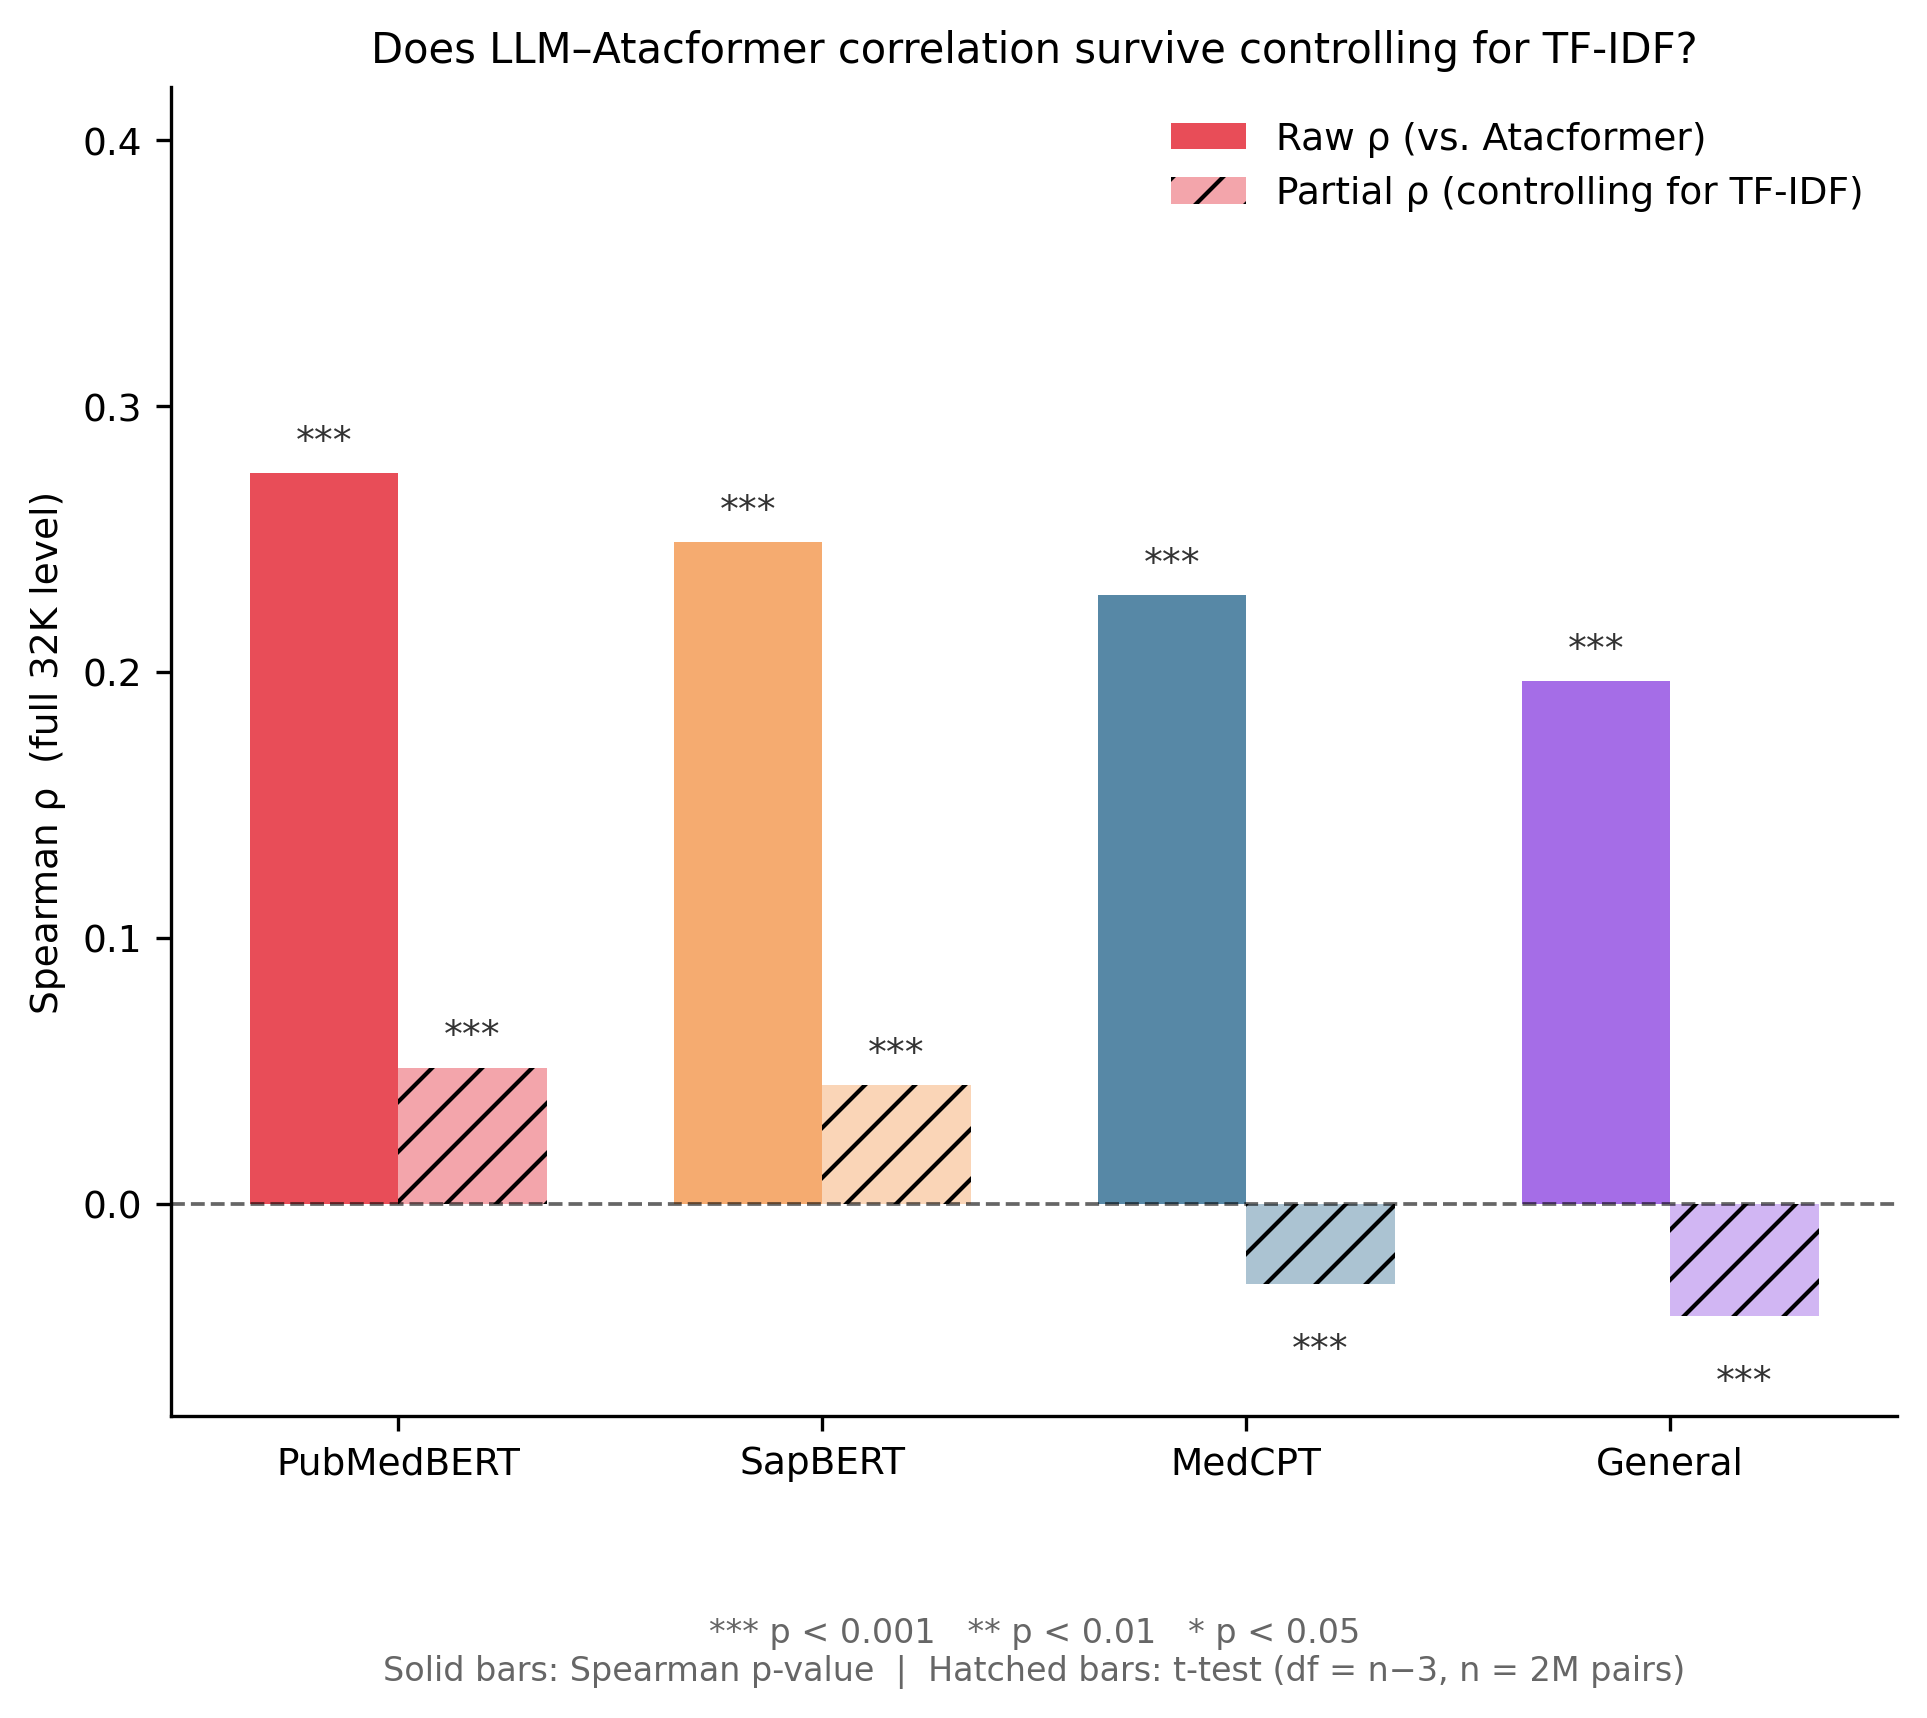
\includegraphics[width=\columnwidth]{fig4a.png}
  \caption{Raw Spearman $\rho$ vs.\ Atacformer (solid bars) and partial
  Spearman $\rho$ after controlling for TF-IDF (hatched bars), full
  32,245-experiment level. PubMedBERT and SapBERT retain positive partial
  correlations; MedCPT and General do not.}
  \label{fig:decomp}
\end{figure}

\begin{figure}[!t]
  \centering
  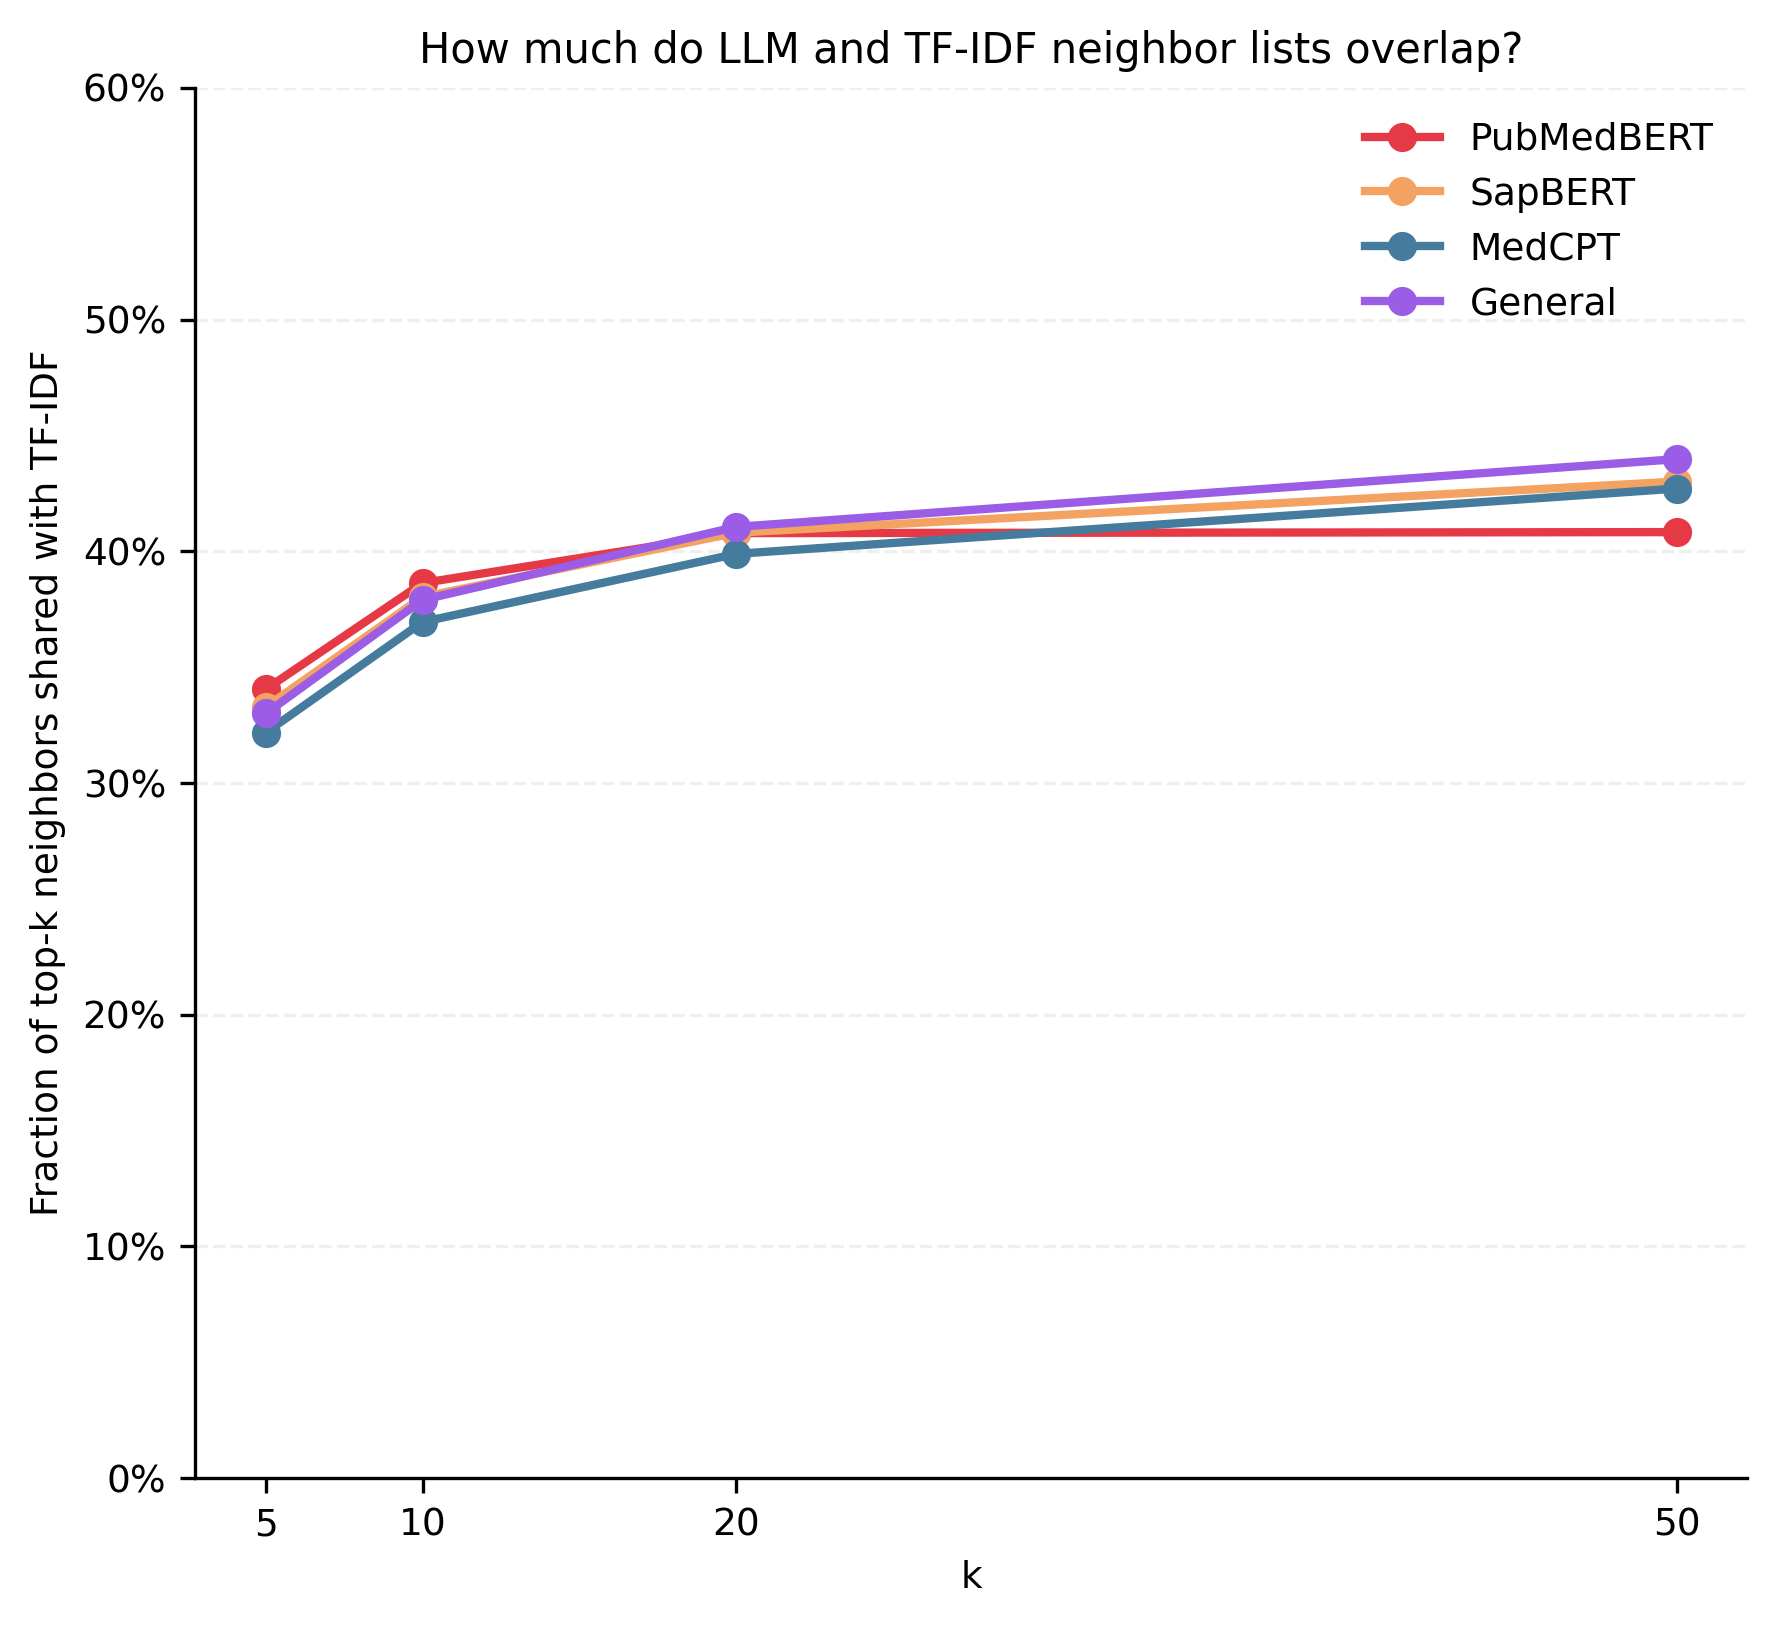
\includegraphics[width=\columnwidth]{fig4b.png}
  \caption{Fraction of top-$k$ LLM nearest neighbors shared with TF-IDF.
  Roughly $\sim$33\% of nearest neighbors are shared at $k=5$ across all four
  models, indicating two-thirds of each LLM's local structure is distinct from TF-IDF.}
  \label{fig:decomp_b}
\end{figure}

\begin{figure*}[!t]
  \centering
  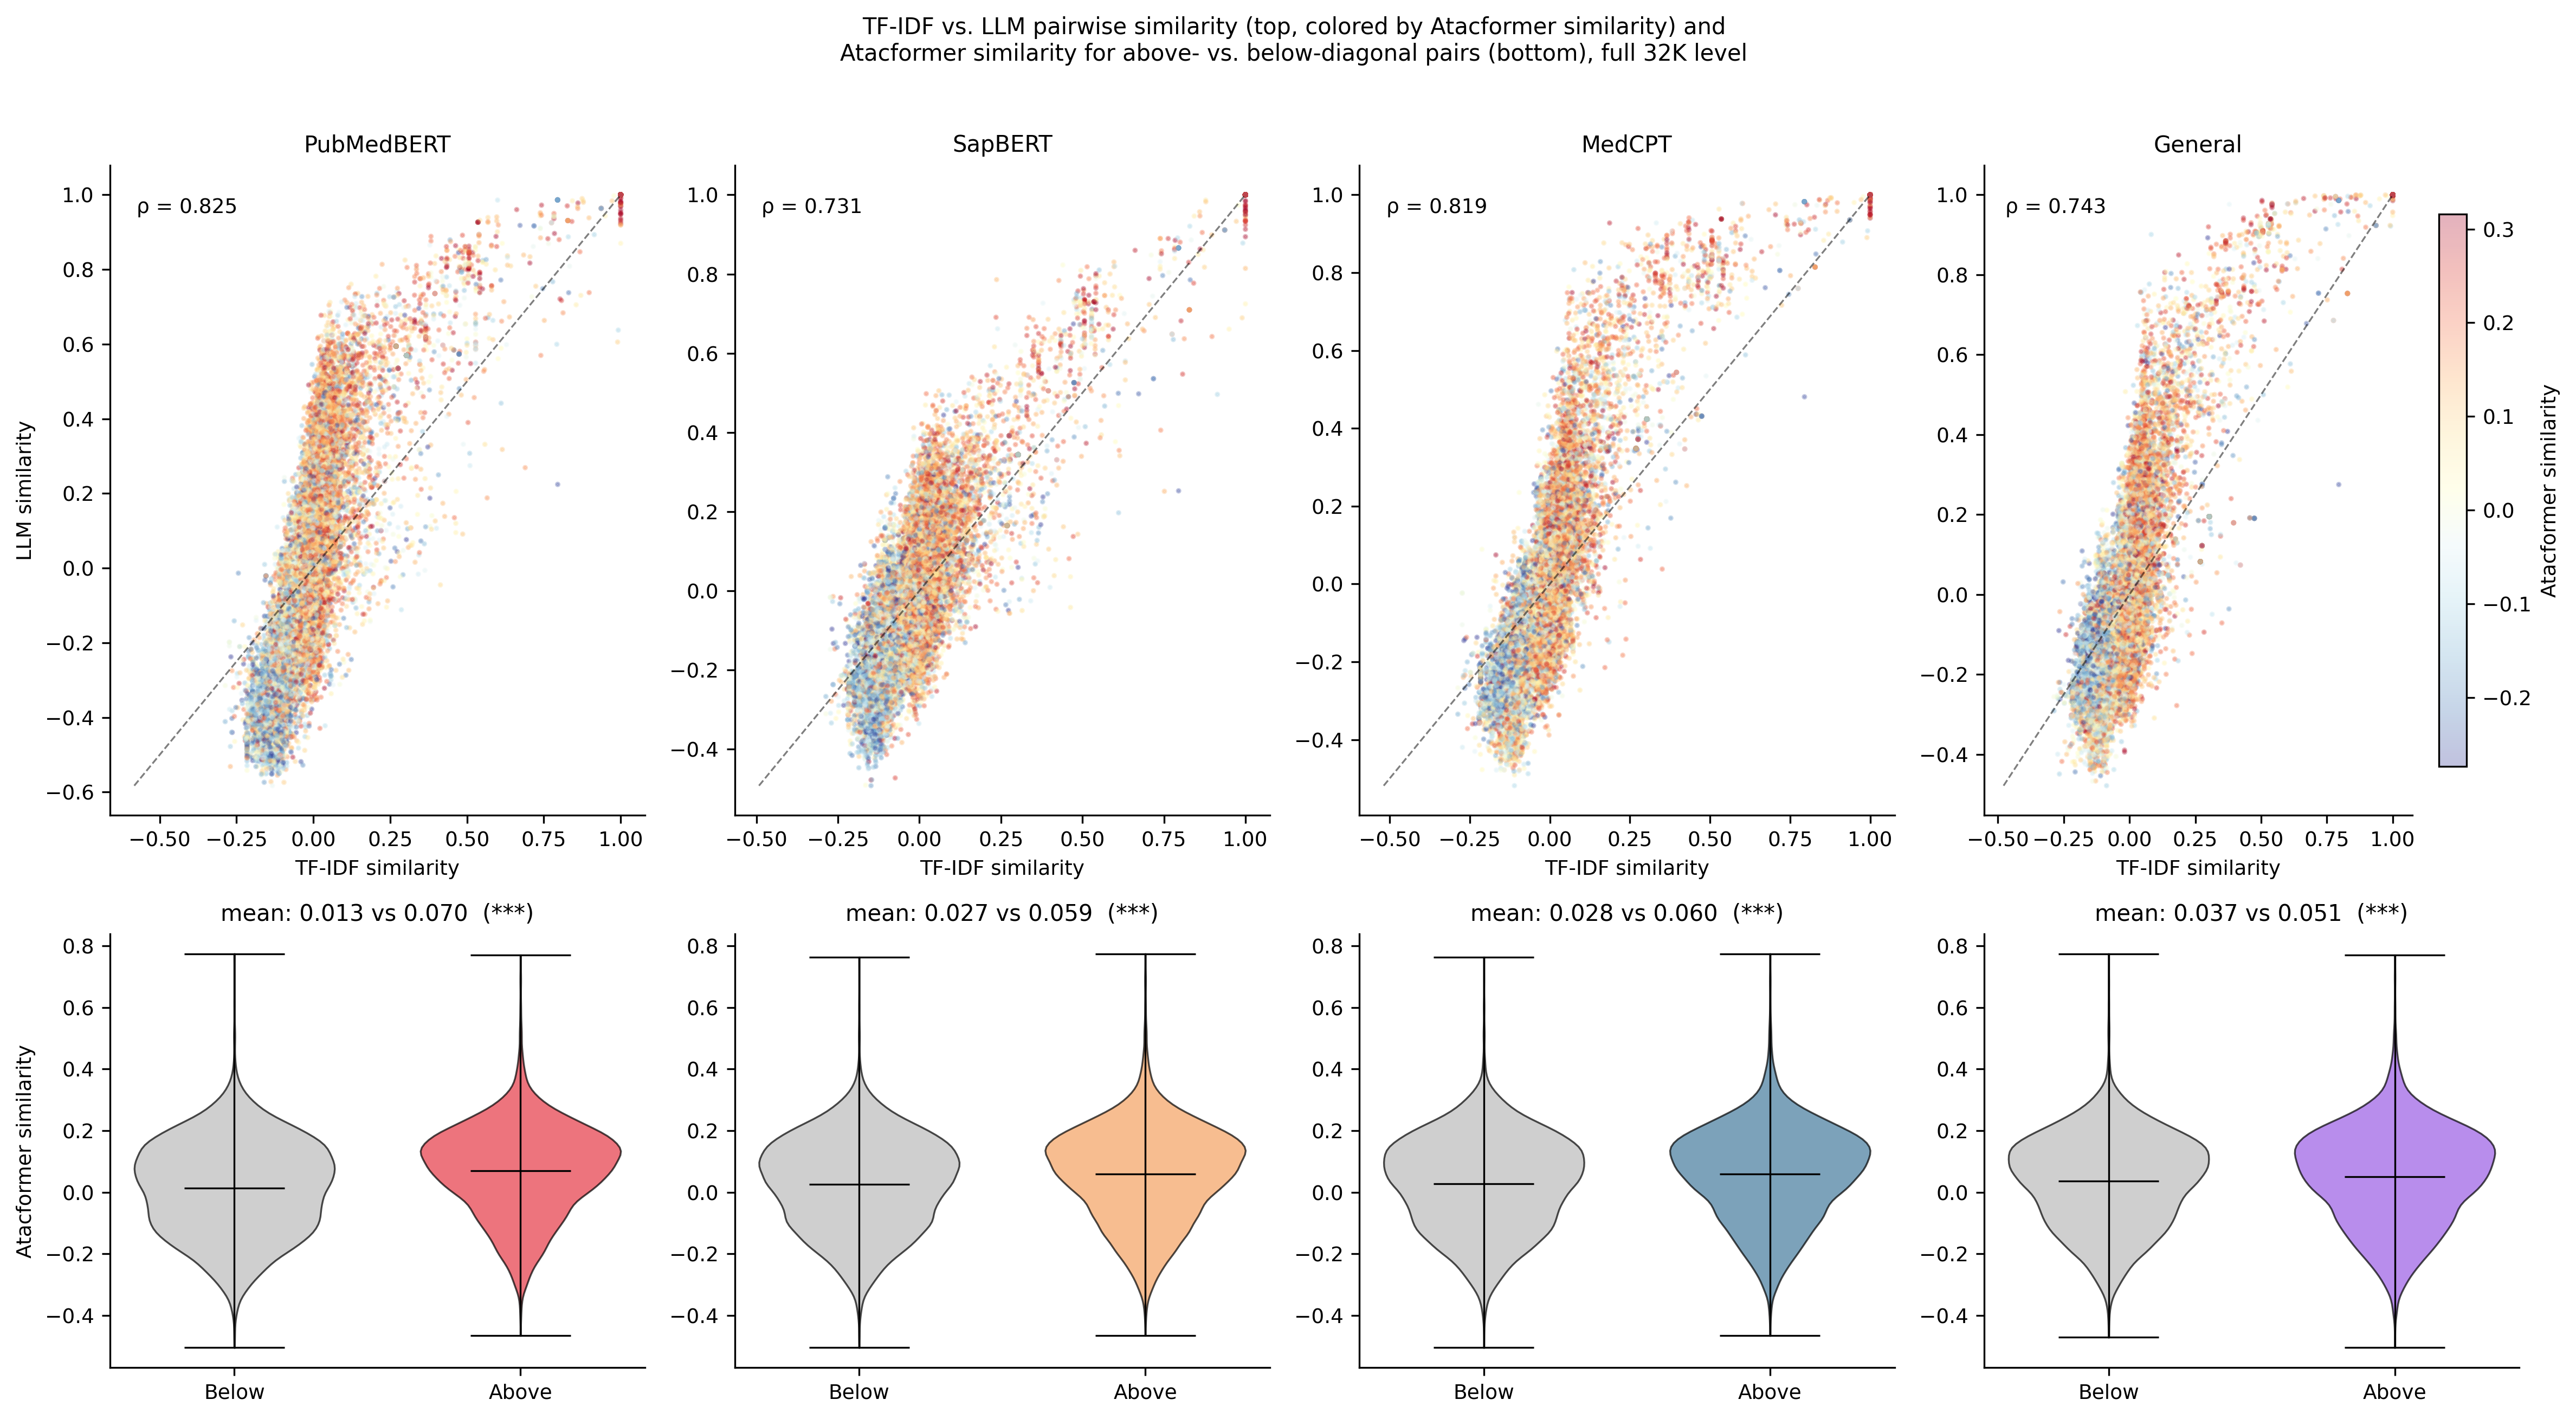
\includegraphics[width=\linewidth]{figS3.png}
  \caption{Top: Pairwise similarity scatter: TF-IDF
  ($x$-axis) vs.\ each LLM ($y$-axis) for 25,000 randomly sampled experiment
  pairs, colored by Atacformer similarity. Points above the diagonal indicate
  pairs the LLM scores higher than TF-IDF; points below indicate the reverse.
  Bottom: violin plots of Atacformer similarity for below- vs.\ above-diagonal
  pairs from the panel above (horizontal bars mark the mean). For all four
  models, above-diagonal pairs have significantly higher mean Atacformer
  similarity than below-diagonal pairs (Welch's $t$-test, unequal variances;
  PubMedBERT: 0.070 vs.\ 0.013, $t=29.96$, $p=9.6\times10^{-194}$, Cohen's
  $d=0.38$; SapBERT: 0.059 vs.\ 0.027, $p=6.1\times10^{-65}$, $d=0.22$; MedCPT:
  0.060 vs.\ 0.028, $p=3.4\times10^{-61}$, $d=0.21$; general-purpose encoder:
  0.051 vs.\ 0.037, $p=3.6\times10^{-13}$, $d=0.09$). This confirms that
  above-diagonal pairs -- where the LLM scores similarity higher than TF-IDF
  -- carry warmer Atacformer colors, consistent with these models capturing
  chromatin-relevant semantic associations beyond keyword overlap, with the
  effect strongest for PubMedBERT.}
  \label{fig:s3}
\end{figure*}

\FloatBarrier
\subsection{Text Embeddings Share Local Structure with RP but Not Atacformer}

Despite statistically significant global rank correlations, top-$k$
neighborhood overlap between text models and Atacformer was universally low:
at $k = 5$, full-text models shared only 2--3\% of nearest neighbors with
Atacformer (Fig.~\ref{fig:topk}). To test whether this reflects a
fundamental limitation of text embeddings or an Atacformer-specific property,
we repeated the analysis using RP as the reference
(Fig.~\ref{fig:topk_rp}; see also Fig.~\ref{fig:s2}).

The same full-text models shared 20--23\% of nearest neighbors with RP at
$k = 5$---a seven-fold increase relative to Atacformer (PubMedBERT: 22.5\%;
SapBERT: 22.1\%; General: 21.4\%; MedCPT: 19.8\%). This dissociation
persisted across all values of $k$ tested. Cell-type-name-only models showed
intermediate overlap with RP ($\sim$7\% at $k = 5$), substantially higher
than their Atacformer overlap ($\sim$1\%), consistent with RP partially
encoding cell type identity through gene activation proximity.

We interpret this dissociation as follows. RP encodes a gene-activation-weighted
summary of chromatin accessibility that closely tracks cell type identity.
Text embeddings similarly cluster experiments by cell type through shared
metadata vocabulary. Atacformer, by contrast, encodes the detailed peak-level
chromatin accessibility landscape, capturing biological variation within and
across cell types not reflected in text metadata. While Atacformer's broader
similarity ordering partially correlates with text globally, its local
neighborhoods are not predictable from metadata alone. These results show that
text metadata is a viable proxy for cell-type-level clustering but
not for the chromatin-specific similarity landscape encoded by
Atacformer.

\begin{figure}[!t]
  \centering
  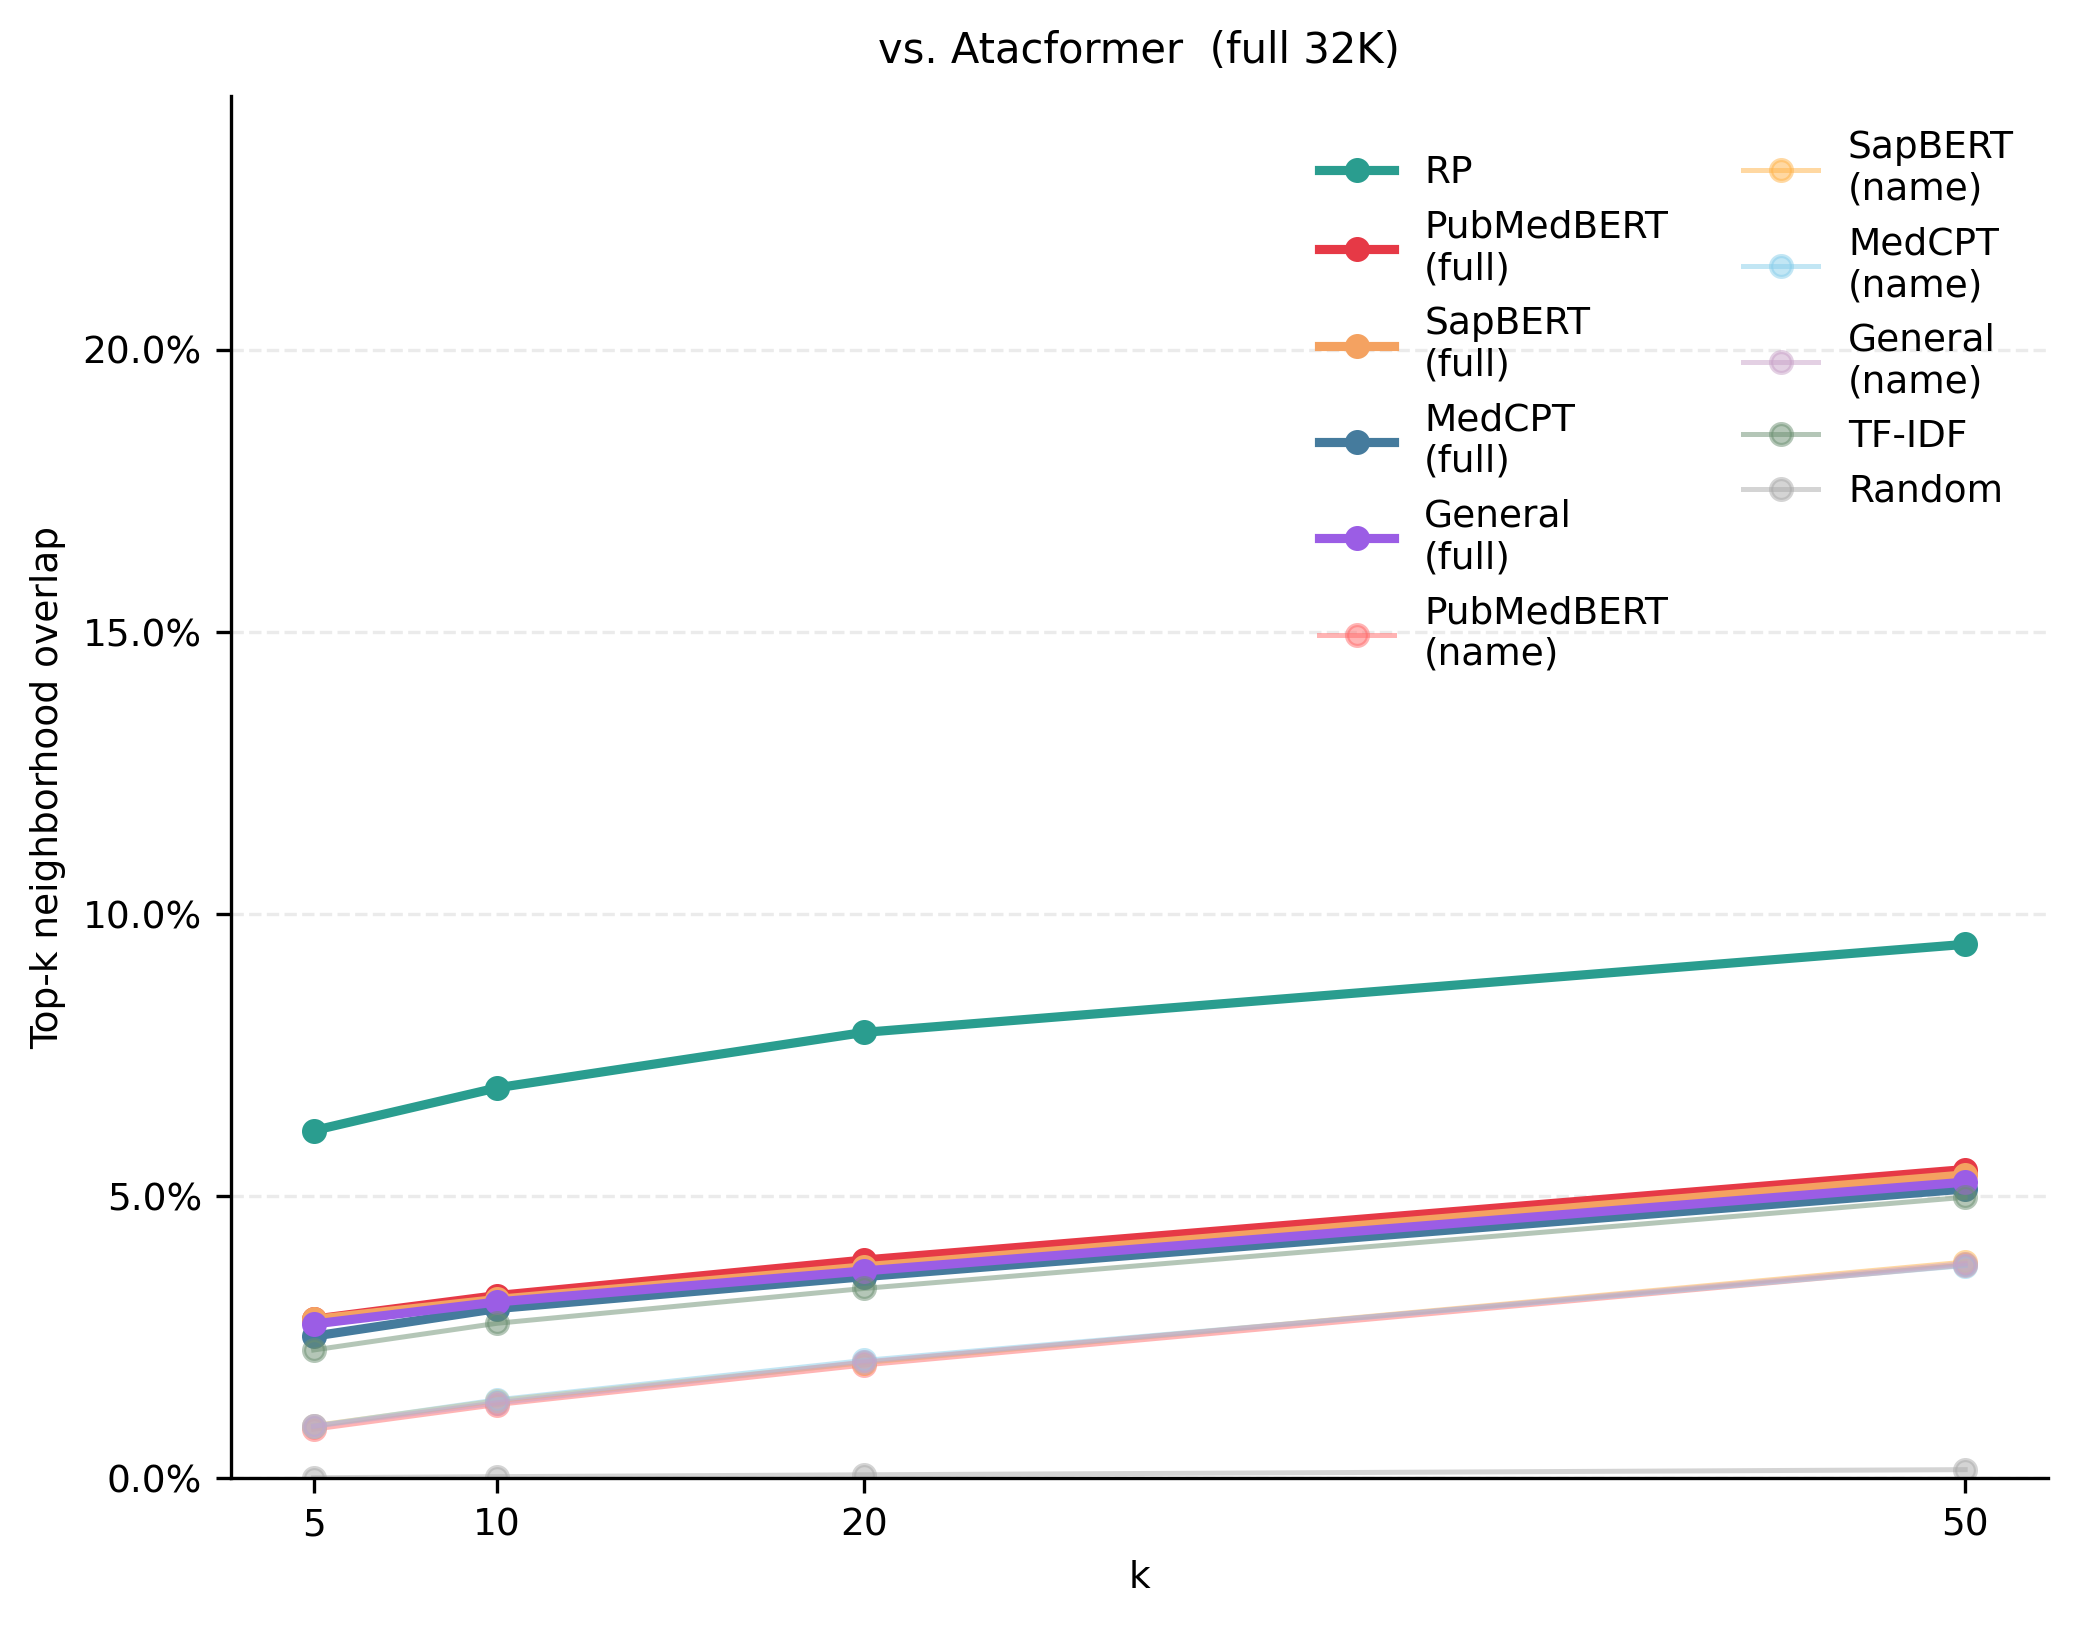
\includegraphics[width=\columnwidth]{fig3a.png}
  \caption{Top-$k$ neighborhood overlap vs.\ Atacformer at the full
  32,245-experiment scale. Full-text models share only $\sim$2--3\% of
  nearest neighbors with Atacformer at $k=5$.}
  \label{fig:topk}
\end{figure}

\begin{figure}[!t]
  \centering
  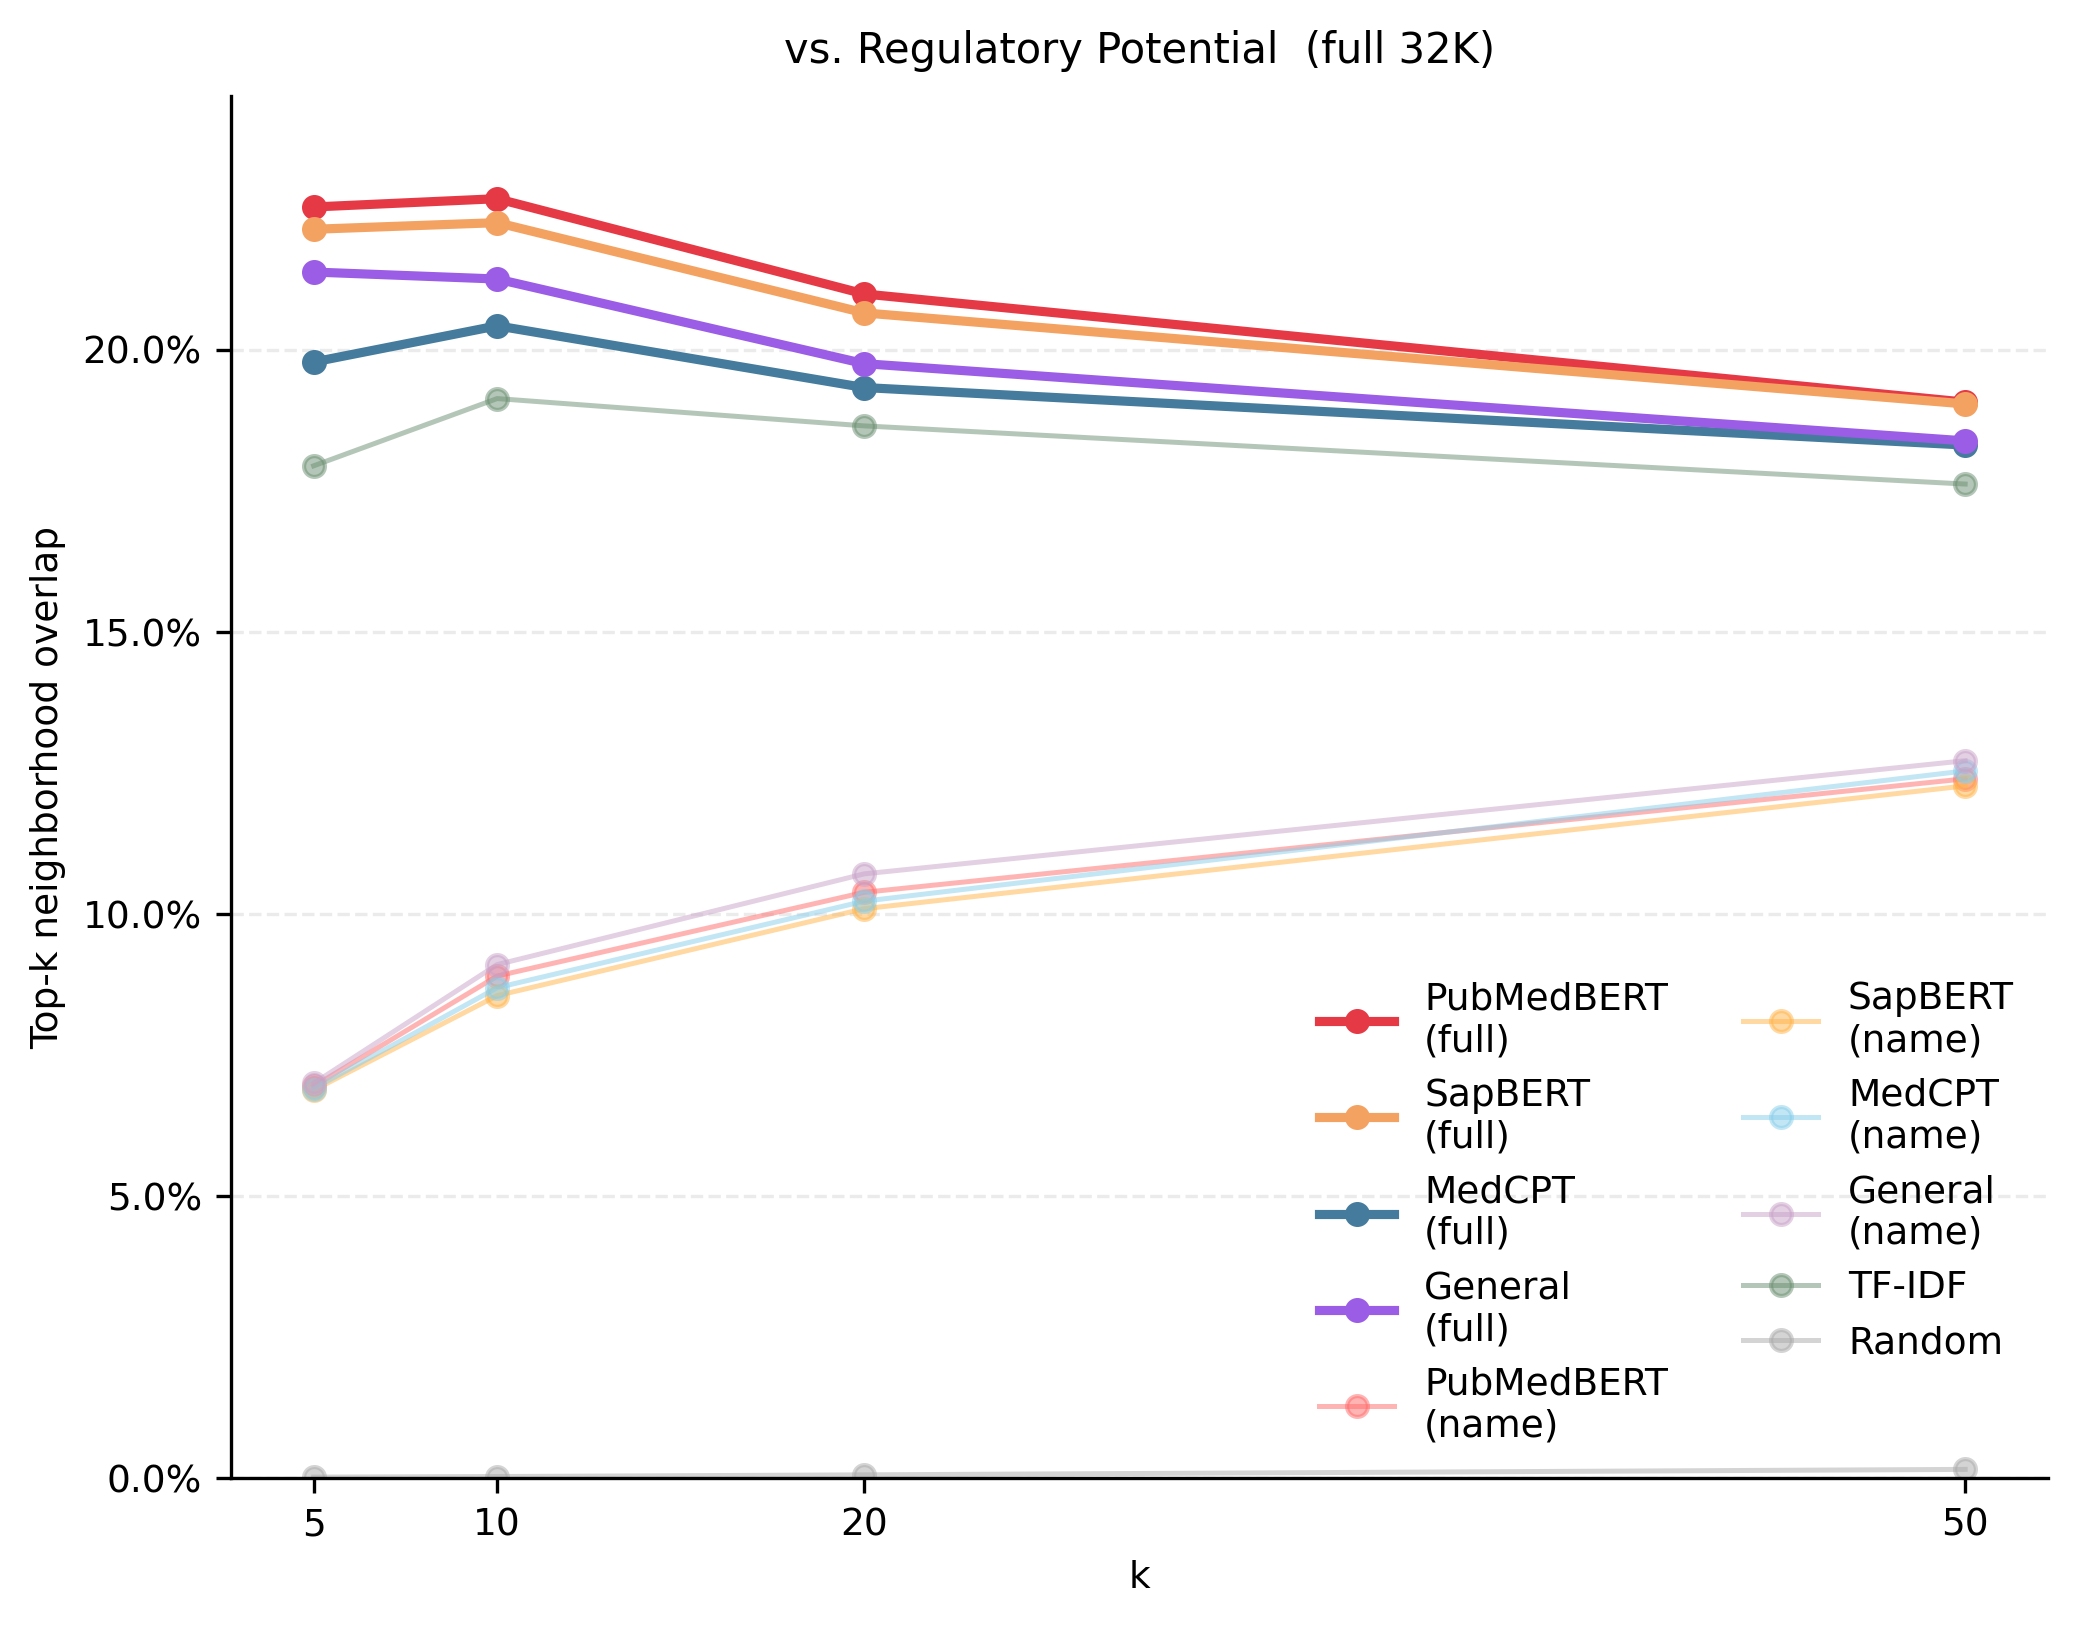
\includegraphics[width=\columnwidth]{fig3b.png}
  \caption{Top-$k$ neighborhood overlap vs.\ regulatory potential (RP) at the
  full 32,245-experiment scale. Full-text models share $\sim$20--23\% of nearest
  neighbors with RP at $k=5$---a seven-fold increase relative to Atacformer.}
  \label{fig:topk_rp}
\end{figure}

\begin{figure*}[!t]
  \centering
  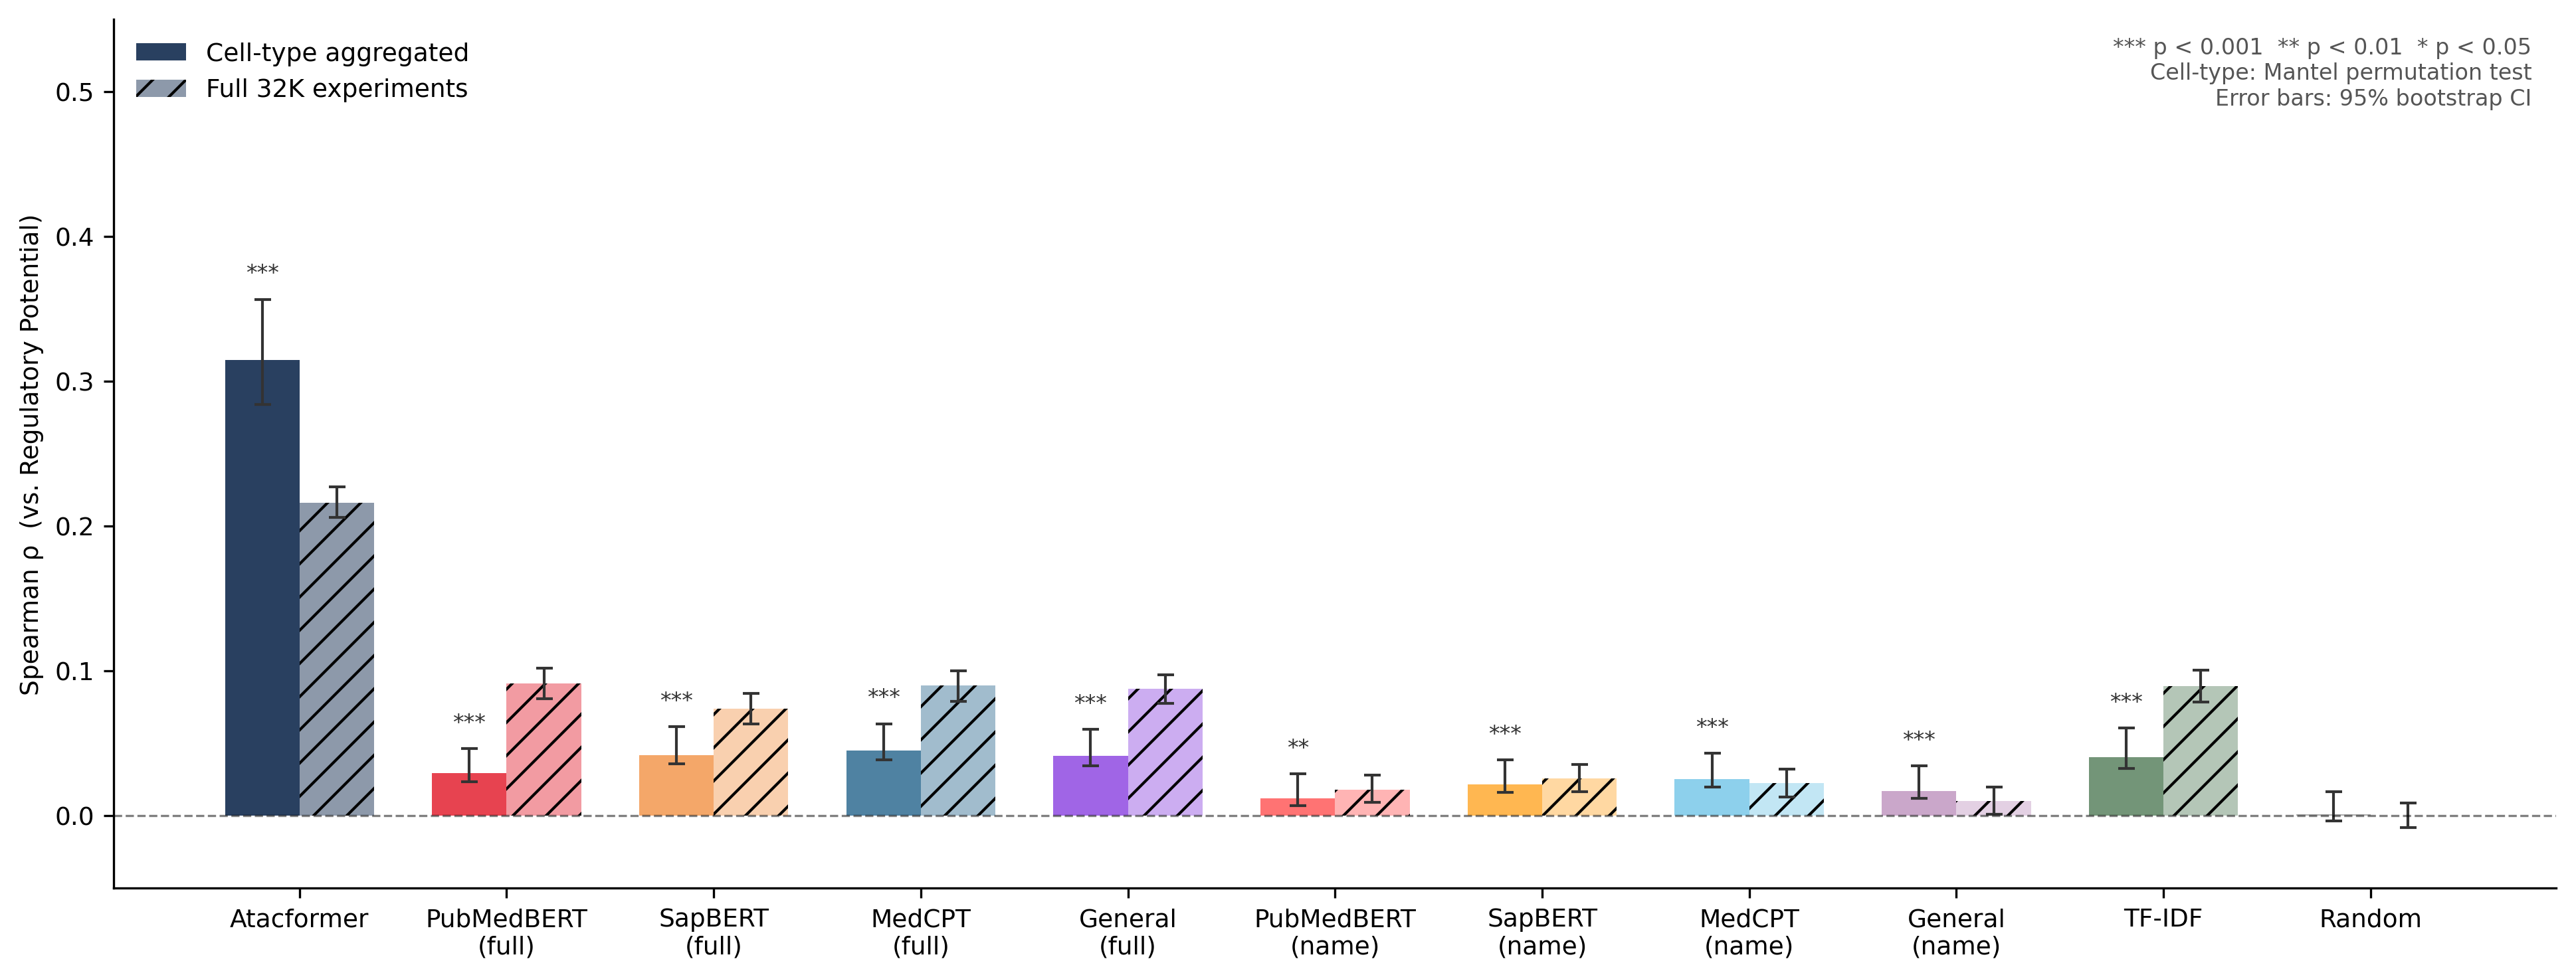
\includegraphics[width=\linewidth]{figS2.png}
  \caption{Spearman rank correlation between each embedding
  type and regulatory potential (RP). Analogous to Table~\ref{tab:spearman}
  with RP as reference. Error bars show 95\% bootstrap confidence intervals;
  significance markers (Mantel permutation test) are shown for the
  cell-type-aggregated bars only.}
  \label{fig:s2}
\end{figure*}

To test this directly, we computed the within-cell-type similarity for each
embedding type---the mean pairwise cosine similarity among experiments sharing
a cell-type label (947 cell types with $\geq 2$ experiments). RP experiments
of the same cell type are highly self-similar (median similarity 0.50),
whereas Atacformer experiments of the same cell type are markedly less
self-similar (median 0.16; Wilcoxon signed-rank $p = 9.1 \times 10^{-140}$),
with Atacformer similarity lower than RP for 91.6\% of cell types
(Fig.~\ref{fig:s4}). This confirms that RP representations are dominated by
cell-type identity, while Atacformer retains substantial within-cell-type
heterogeneity that text-derived metadata cannot resolve.

\begin{figure}[!t]
  \centering
  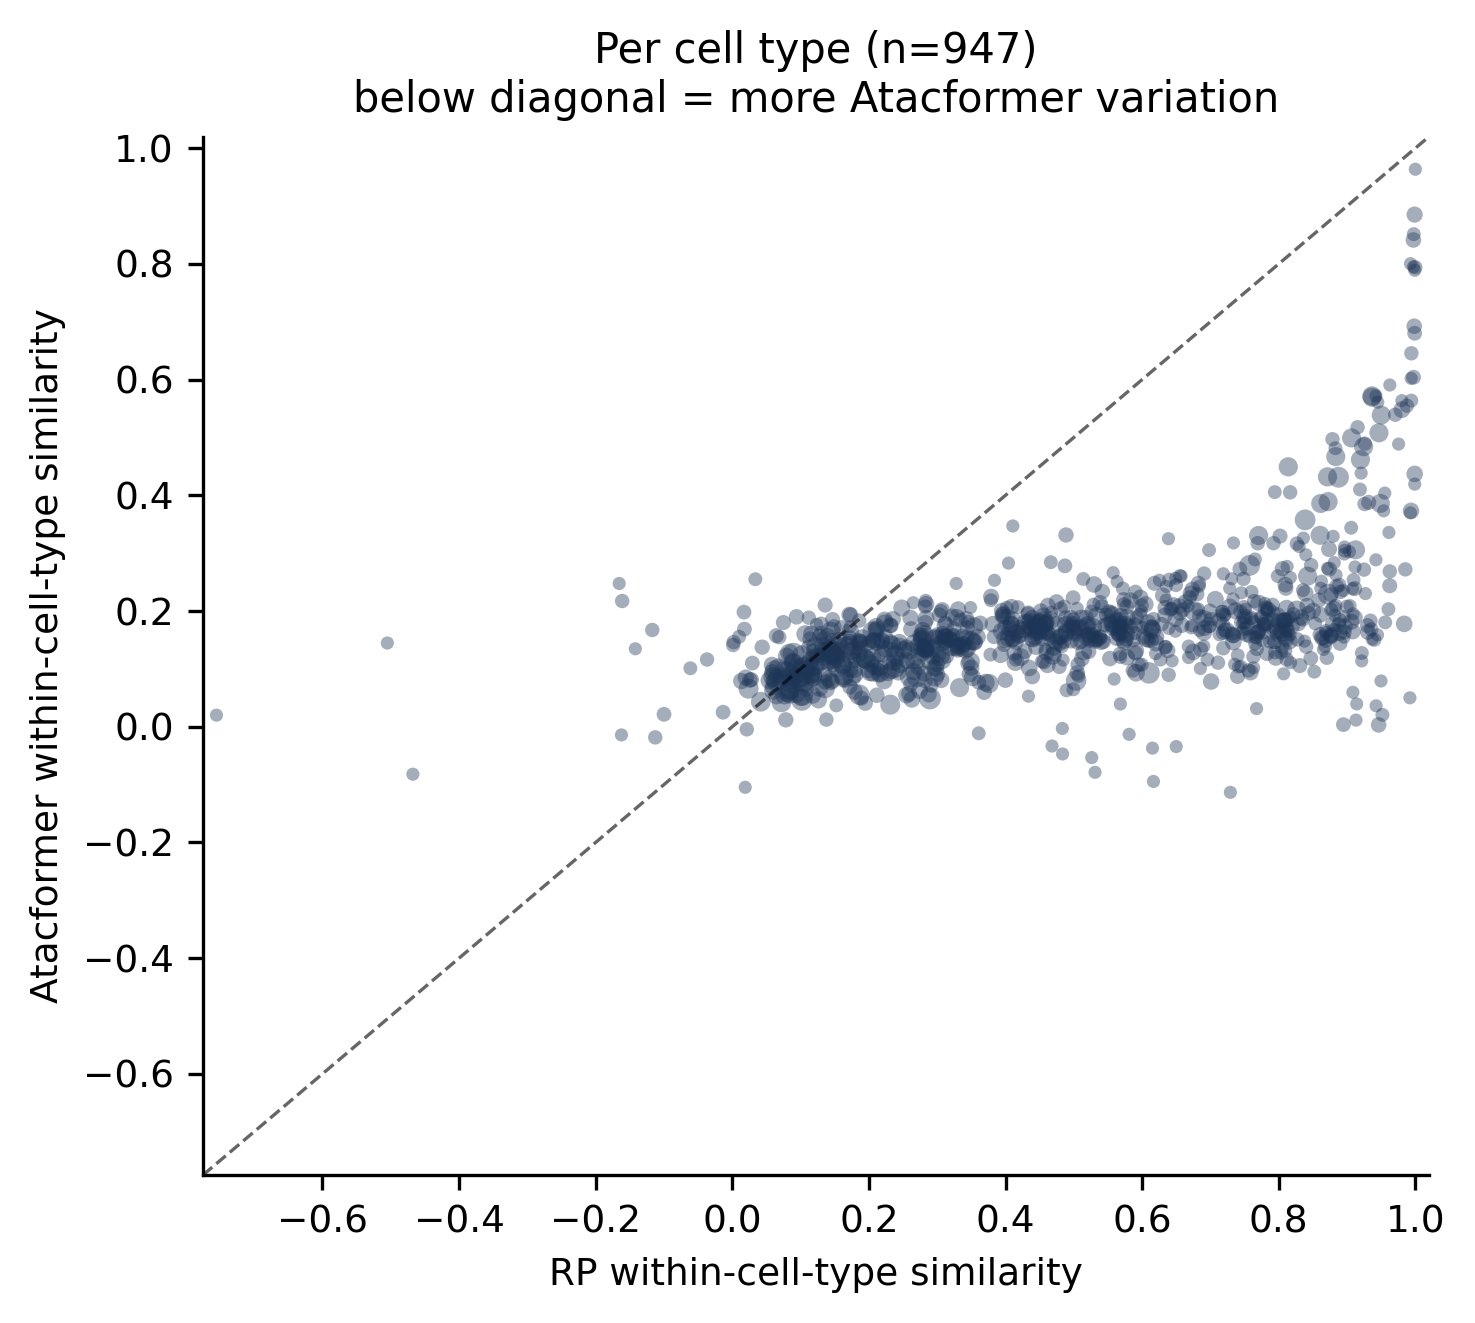
\includegraphics[width=\columnwidth]{figS4a.png}
  \caption{Per-cell-type within-cell-type similarity for Atacformer
  vs.\ regulatory potential (RP), computed as mean pairwise cosine similarity
  among experiments sharing a cell-type label (947 cell types with
  $\geq 2$ experiments). Points below the diagonal indicate higher
  within-cell-type variation for Atacformer than RP.}
  \label{fig:s4}
\end{figure}

\begin{figure}[!t]
  \centering
  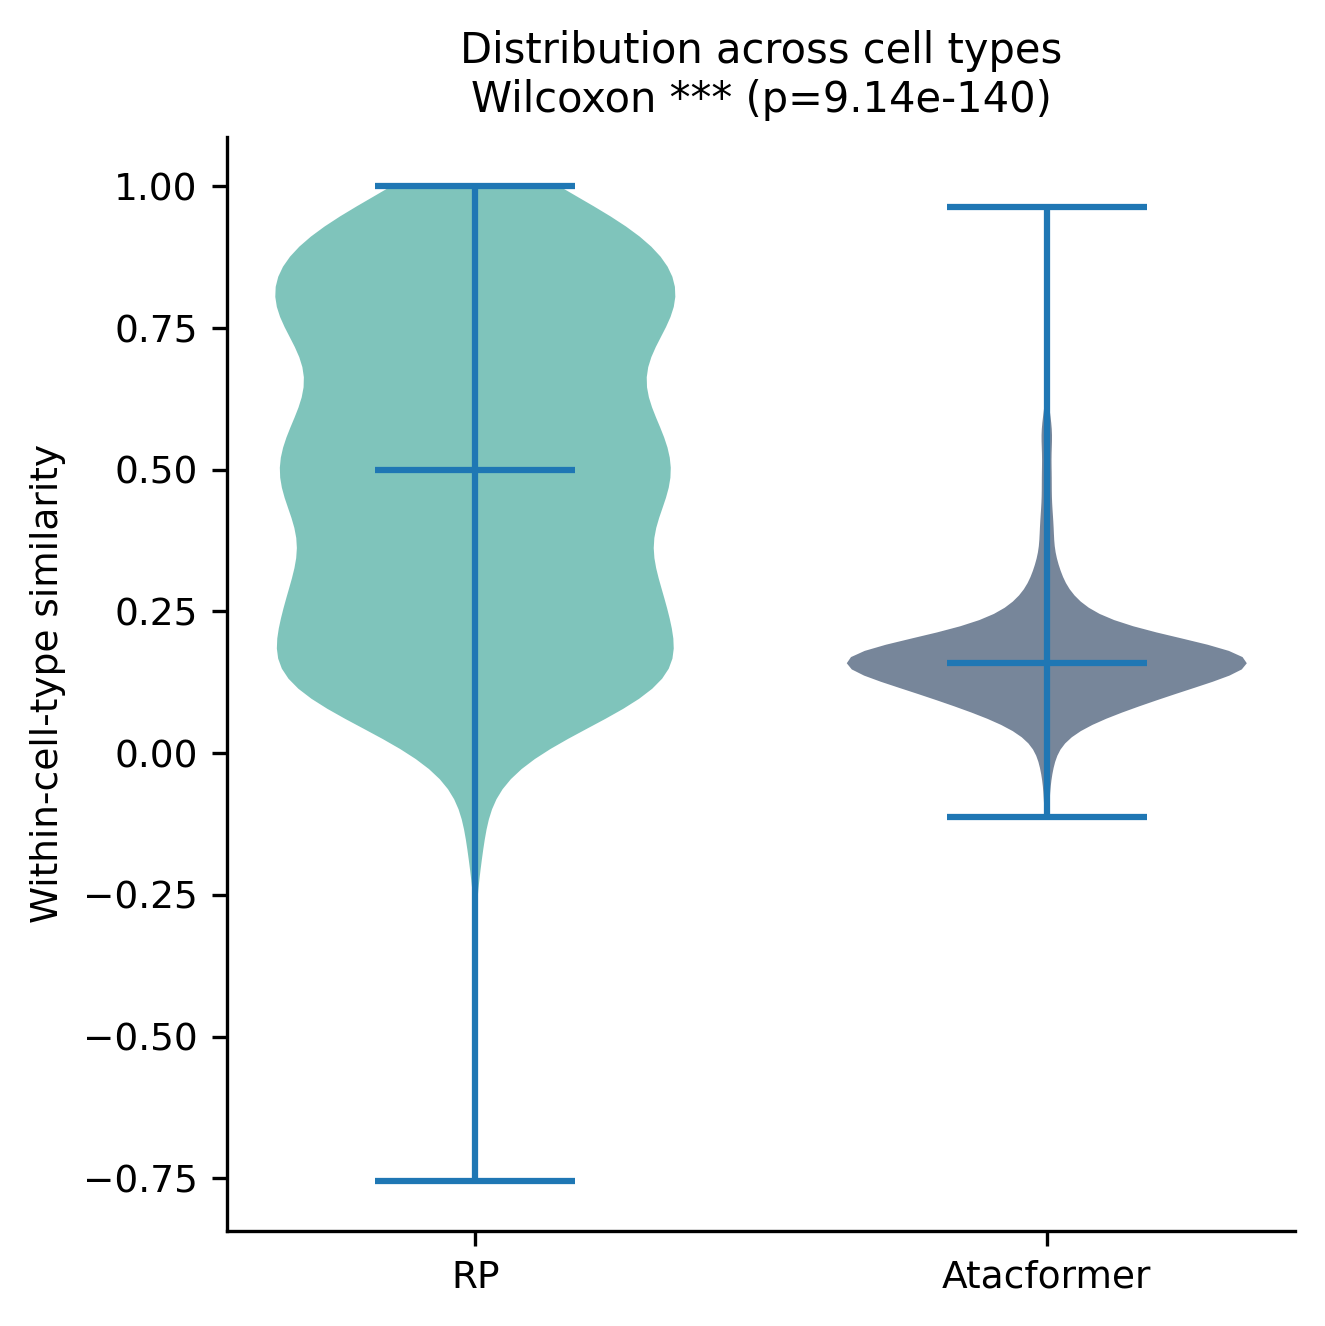
\includegraphics[width=\columnwidth]{figS4b.png}
  \caption{Distribution of within-cell-type similarity across cell types
  (Wilcoxon signed-rank test). RP experiments are highly self-similar
  within cell type (median 0.50); Atacformer experiments are markedly less
  so (median 0.16), reflecting substantial within-cell-type heterogeneity.}
  \label{fig:s4b}
\end{figure}

To illustrate this concretely, we examined pairs of experiments with high
chromatin similarity (top 5\%) but low TF-IDF similarity (below median;
Tables~\ref{tab:qual_atac}--\ref{tab:qual_rp}). For Atacformer, these pairs
link experiments with entirely different cell-type labels---e.g., the lung
cancer line NCI-H1299 and CD4+ T cells (Atacformer similarity 0.37, TF-IDF
similarity $-0.20$), or NCI-H1648 and iPSC-derived neural cells ($0.31$
vs.\ $-0.20$). RP shows the same pattern at higher similarity values, e.g.,
NCI-H2347 and PBMC (RP similarity 0.88, TF-IDF similarity $-0.18$). In each
case, the text descriptions share essentially no vocabulary, yet the
chromatin profiles are substantially more similar than a typical pair drawn
from the dataset.

\begin{table}[!t]
  \centering
  \footnotesize
  \caption{Experiment pairs: high Atacformer similarity, low TF-IDF
  similarity (top 5\% / below-median, 58,128 pairs). Cell-type labels
  differ entirely, illustrating chromatin similarity unpredictable from
  metadata.}
  \label{tab:qual_atac}
  \setlength{\tabcolsep}{4pt}
  \begin{tabular}{llcc}
    \toprule
    Cell type A & Cell type B & Atac. & TFIDF \\
    \midrule
    NCI-H1299            & CD4+ T cells              & $0.374$ & $-0.196$ \\
    iPSC derived cells   & PC-9                      & $0.361$ & $-0.176$ \\
    NCI-H1648            & iMeLCs                    & $0.312$ & $-0.214$ \\
    (unlabeled)          & CD4+ T cells              & $0.398$ & $-0.147$ \\
    NCI-H1648            & iPSC neural cells         & $0.307$ & $-0.204$ \\
    (unlabeled)          & IMR-90                    & $0.309$ & $-0.188$ \\
    (unlabeled)          & MV-4-11                   & $0.331$ & $-0.156$ \\
    (unlabeled)          & Neural crest cells        & $0.310$ & $-0.179$ \\
    iPSC derived cells   & Jurkat                    & $0.318$ & $-0.164$ \\
    (unlabeled)          & DND-41                    & $0.316$ & $-0.161$ \\
    \bottomrule
  \end{tabular}
\end{table}

\begin{table}[!t]
  \centering
  \footnotesize
  \caption{Experiment pairs: high RP similarity, low TF-IDF similarity,
  selected analogously to Table~\ref{tab:qual_atac}.}
  \label{tab:qual_rp}
  \setlength{\tabcolsep}{4pt}
  \begin{tabular}{llcc}
    \toprule
    Cell type A & Cell type B & RP & TFIDF \\
    \midrule
    iPSC derived cells & K-562           & $0.885$ & $-0.221$ \\
    NCI-H2347          & PBMC            & $0.884$ & $-0.181$ \\
    RERF-LC-Ad1        & XG-6            & $0.851$ & $-0.224$ \\
    (unlabeled)        & PKC19           & $0.901$ & $-0.171$ \\
    iPSC derived cells & T-47D           & $0.874$ & $-0.185$ \\
    (unlabeled)        & B-cell leukemia & $0.891$ & $-0.170$ \\
    NCI-H1648          & B cells         & $0.859$ & $-0.181$ \\
    NCI-H1703          & CD4+ T cells    & $0.851$ & $-0.186$ \\
    NCI-H1299          & CD4+ T cells    & $0.833$ & $-0.196$ \\
    (unlabeled)        & ES cells        & $0.916$ & $-0.154$ \\
    \bottomrule
  \end{tabular}
\end{table}

\FloatBarrier
% ── Discussion ────────────────────────────────────────────────────────────────
\section{Discussion}

Our results establish quantitative bounds on the utility of experimental
metadata as a proxy for ATAC-seq chromatin similarity, and reveal a nuanced
picture of when language model pretraining adds value beyond simple vocabulary
statistics.

The dominant finding is that vocabulary overlap---as measured by TF-IDF---
accounts for the majority of the text--Atacformer correlation. TF-IDF achieves
the highest raw Spearman correlation at the full scale ($\rho = 0.300$) and
fully explains the Atacformer alignment of both the general-purpose encoder and
MedCPT. Taken at face value, this implies that experimental metadata primarily
informs chromatin similarity through shared terminology, not semantic
understanding.

The partial correlation analysis (Section~3.2) complicates this picture.
PubMedBERT ($\Delta\rho = +0.051$) and SapBERT ($\Delta\rho = +0.045$) retain
small but non-zero positive partial correlations with Atacformer after
controlling for TF-IDF, whereas MedCPT ($\Delta\rho = -0.030$) and the
general-purpose encoder ($\Delta\rho = -0.042$) do not. Because PubMedBERT,
SapBERT, and MedCPT are all derived from the same PubMedBERT-pretrained base,
this divide is more plausibly attributable to fine-tuning objective than to
differences in base biomedical-literature pretraining: SapBERT's UMLS
synonym-alignment fine-tuning preserves a notion of general semantic
similarity, whereas MedCPT's retrieval-relevance fine-tuning on search-click
logs may not. We emphasize that these partial correlations are small in
absolute terms and establish only that a non-zero residual exists---not that
it constitutes biologically meaningful ``semantic understanding.''

The global-versus-local dissociation between Atacformer and RP as reference
structures reveals a complementary insight. Text embeddings capture cell-type-level
clustering (which RP also encodes) but not the within-cell-type chromatin
variation that Atacformer encodes. Text metadata may therefore support
coarse-grained retrieval but should not substitute for chromatin similarity in
fine-grained applications.

A central limitation of this study is that Atacformer and RP are both treated
as proxies for ``true'' chromatin biology, but neither has been independently
validated against an external biological ground truth. Both are mathematical
transforms of the same underlying ChIP-Atlas peak-call data: RP is a
hand-specified, gene-centric exponential-decay summary of peak-to-TSS
distances, while Atacformer is a learned, peak-token-based embedding whose
inductive biases have not been independently characterized. Consequently, RP
and Atacformer are not independent reference structures---RP can be viewed as
a structured, gene-centric compression of much of the same peak-level
information that Atacformer encodes more flexibly. All conclusions in this
study about what text embeddings do or do not capture are therefore bounded by
the assumption that Atacformer and RP faithfully represent the chromatin
biology they are intended to proxy; to the extent that either reference
carries its own biases or blind spots, our measurements of text--chromatin
agreement inherit those biases.

Additional limitations include the heterogeneous quality of ChIP-Atlas
experiments, the restriction to metadata fields available in ChIP-Atlas, and
the absence of multimodal embeddings combining text and chromatin signals.
Future work could explore whether fine-tuned text encoders trained to directly
predict chromatin similarity, or retrieval-augmented multimodal approaches,
could narrow the gap. The non-zero partial correlations for PubMedBERT and
SapBERT suggest a residual signal that warrants further characterization,
though establishing whether it reflects genuine biological semantics---rather
than, e.g., shared structure with the reference embeddings themselves---would
require validation against an independent biological ground truth.

% ── Acknowledgements ──────────────────────────────────────────────────────────
\section*{Acknowledgements}

This work was supported by NVIDIA Corporation through its academic grant
program via the provision of an NVIDIA DGX Spark system.

% ── References ────────────────────────────────────────────────────────────────
\bibliographystyle{IEEEtran}
\bibliography{references}

\end{document}
